% SIAM Article Template
\documentclass{article}
\usepackage{algorithm}
\usepackage{algorithmic}
\usepackage{subfig}
\usepackage{forest}
\usepackage[section]{placeins}
\usepackage[export]{adjustbox}
\usepackage{amsmath}
\usepackage{amsfonts}
\usepackage[framed,numbered,autolinebreaks,useliterate]{mcode}
\usepackage{amsthm}
\usepackage{cite}
\usepackage[margin=1.5in]{geometry}
\DeclareMathOperator*{\argmin}{argmin}
\DeclareMathOperator*{\osc}{osc}


\newtheorem{theorem}{Theorem}[section]
\newtheorem{roughtheorem}{Rough Theorem}[section]
\newtheorem{corollary}{Corollary}[theorem]
\newtheorem{lemma}[theorem]{Lemma}
\newtheorem{assumption}{Assumption}
\newcommand{\lp}{\left(}
\newcommand{\rp}{\right)}

\newcommand{\R}{\mathbb{R}}
\newcommand{\N}{\mathbb{N}}
\newcommand{\Z}{\mathbb{Z}}
\newcommand{\Q}{\mathbb{Q}}
\newcommand{\C}{\mathbb{C}}
\newcommand\supp{\mathop{\rm supp}}

\newcommand{\vect}[1]{\mathbf{#1}}
\DeclareMathOperator{\vecm}{vec}
\newcommand{\plotwidth}{0.45}
\newcommand{\WRP}{\par\qquad\(\hookrightarrow\)\enspace}

%%%%% custom commands for this paper
\newcommand{\nmax}{n_{\text{max}}}
\newcommand{\child}[1]{c\textsubscript{#1}}
\newcommand{\weight}[1]{w\textsubscript{#1}}
\newcommand{\bound}[1]{b\textsubscript{#1}}

\newcommand{\dm}{d_{\text{max}}}
%%%%%

\begin{document}

\section{ND PU Structure}
\label{Structsec}
Since we are thinking of mixing methods for our PU approximation, it seems we should think more about the modularity of the method. My first thought is to have an abstract PATCH $\nu$ with properties
\begin{itemize}
\item domain($\nu$):= domain of $\nu$
\item boundaryIndex($\nu$):= boundary index of points of $\nu$
\item length($\nu$):= length of $\nu$
\item dim($\nu$):= dimension of the space domain($\nu$) lies in
\end{itemize}
with methods
\begin{itemize}
\item points($\nu$):=returns the points of $\nu$
\item evalf($\nu$,x):=evaluates the approximate for $\nu$ at $x$.
\item sample($\nu$,f(x)):= samples $f(x)$ at the leaves of $\nu$
\end{itemize}

\begin{figure}[!h]
\centering
     \begin{forest}
[ PATCH
    [ LEAFPATCH 
    [ RBFPATCH
    ] 
    [ CHEBPATCH
    ]]
    [ PUPATCH 
    [ PURECTPATCH ]
    ]
]
\end{forest}
\caption{Object structure for the patches.}
\end{figure}
Here RBFPATCH and CHEBPATCH would be used as leaves where RECTPUPATCH would be used for nonleaves. A PUPATCH has additional properties
\begin{itemize}
\item \child{0}($\nu$), \child{1}($\nu$):= two PATCH children
\item \weight{0}($\nu$), \weight{1}($\nu$):= weights used for children
\end{itemize}
The methods would be defined, ignorant of the type of patches the children are. As an example, the evalf($\nu$,x) method would be defined similarly as before where the leaves are assumed to be type PATCH (this objects would have there own evalf method). By defining different objects for different methods (RBF,CHEB), we can use this generic method for our different cases (a box, arbitrary boundary).

 The leaf patches would be defined for the specific method at the leaves. We next define a method 
\begin{itemize}
\item PATCH $\nu_1$ = splitleaf(LEAFPATCH $\nu$)
\end{itemize}
that returns a PUPATCH with two children if $\nu$ needs to be split, and $\nu$ if it does not to be split. We can then define a refine method for a tree $T$ and its nodes $\nu$.

\begin{algorithm}[!h]
\caption{v=eval($\nu$,$x$)}
\label{alg3}
\begin{algorithmic}
\IF{$\nu$ is a leaf}
\STATE $p$:=interpolant($\nu$)
\STATE v:= $p(x)$
\ELSE
\STATE $v_0,v_1$:=0

\STATE $w_0$:=\weight{0}($\nu$)
\STATE $w_1$:=\weight{1}($\nu$)
\FOR{$k=0,1$}
\IF{$x \in$ domain(\child{k}($\nu$))}
\STATE $v_k$:=eval(\child{k}($\nu$),$x$)
\ENDIF
\ENDFOR
\STATE v := $w_0(x)v_0 + w_1(x)v_1$
\ENDIF
\end{algorithmic}
\end{algorithm}


\begin{algorithm}[!h]
\caption{T = refine($f(x)$)}
\label{alg5}
\begin{algorithmic}
\STATE define $T$ has a tree with single node
\WHILE{$T$ has unrefined leaves}
\STATE sample($T$,$f(x)$)
\IF{root($T$) is a leaf}
\STATE root($T$) = splitleaf(root($T$))
\ELSE
\STATE PUsplit(root($T$))
\ENDIF
\ENDWHILE
\end{algorithmic}
\end{algorithm}

\begin{algorithm}[!h]
\caption{PUsplit($\nu$)}
\label{alg6}
\begin{algorithmic}
\FOR{$k=0,1$}
\IF{\child{k}($\nu$) is a leaf and unresolved}
\STATE \child{k}($\nu$):=splitleaf(\child{k}($\nu$))
\ELSE
\STATE PUsplit(\child{k}($\nu$))
\ENDIF
\ENDFOR
\STATE merge($\nu$)
\end{algorithmic}
\end{algorithm}

\section{Calculating Derivatives and Partition of Unity Weights}

For the ND problem, we intend to evaluate the derivatives instead of constructing differentiation matrices. Suppose we have a method evalf($\nu$,$x$,$dim$,$j$) which evaluates the derivative of order $j$ along dimension $dim$ at $x$. We can compute this simply using the product rule as seen in Algorithm~\ref{alg7}. While this is formulation is simple, it is inefficient. In this formulation we end up repeating calculations for the derivatives of the children of the node. This can be avoided by passing up the evaluations of the approximation and its derivatives up to the desired order.

\begin{algorithm}[!h]
\caption{v = evalf($\nu$,$x$,$dim$,$j$)}
\label{alg7}
\begin{algorithmic}
\STATE $w_0$:=\weight{0}($\nu$)
\STATE $w_1$:=\weight{1}($\nu$)
\STATE v = 0
\FOR{$k=0,1$}
\STATE v = v+$\sum_{i=1}^j \binom{j}{i} \partial_{dim}^{j-1} w_k(x) \text{ evalf(\child{k}($\nu$),$x$,$dim$,$j$)}$
\ENDFOR
\end{algorithmic}
\end{algorithm}

For our method we intend to split only along one dimension. In this case our partition of unity weights need only to depend on the dimension that we are splitting along. Some care must be used when calculating the derivatives; if the dimension we are differentiation along is different than the splitting dimension, the derivative of the weights are zero.

\section{Barycentric Interpolation on ND Chebyshev grids}

Suppose we have a tensor product of Chebyshev grids with points $\{x_i\},\{y_j\}$. Let $\{l_{x_i}(x)\}$, $\{l_{y_i}(x)\}$ be the Lagrange polynomials for points $\{x_i\},\{y_j\}$. We then have the interpolating polynomial for a function $f(x,y)$ is
\begin{equation}
p(x,y) = \sum_j \sum_i l_{y_j}(y) l_{x_i}(x) f(x_i,y_j)
\end{equation}
which can be expressed as
\begin{equation}
p(x,y) = \sum_j l_{y_j}(y) \sum_i l_{x_i}(x) f(x_i,y_j).
\end{equation}
This implies that we can evaluate p(x,y) by:
\begin{itemize}
\item Evaluating $c_j = \sum_i l_{x_i}(x) f(x_i,y_j)$ for all points $\{y_j\}$,
\item and then evaluating $\sum_j l_{y_j}(y) c_j$
\end{itemize}
We can thus evaluate $p(x,y)$ with interpolation methods in one dimension. This is illustrated in Figure~\ref{MULTI_INTERP}.

Chebfun includes a \mcode{bary(x,F)} method which will evaluate the Chebyshev interpolants at \mcode{x} given a sampling \mcode{F}; if \mcode{F} is matrix, the method will compute the Chebyshev interpolants for each of the columns of \mcode{F}. The method can thus be used as is for 2D interpolation. But lets suppose \mcode{F} is $f(x,y,z)$ sampled on a 3D Chebyshev tensor product grid of dimension $n_1 \times n_2 \times n_3$ (i.e., $F$ is a multidimensional array). Lets now suppose we have $\{x_i\},\{y_j\}, \{z_k\}$. Let $\{l_{x_i}(x)\}$, $\{l_{y_i}(x)\},\{l_{z_k}(x)\}$ be the Lagrange polynomials for points $\{x_i\},\{y_j\},\{z_k\}$. Then in-order to evaluate
\begin{equation}
p(x,y,z) = \sum_k l_{z_k}(z) \sum_j l_{y_j}(y)  \sum_i  l_{x_i}(x) f(x_i,y_j,z_k)
\end{equation}
by
\begin{itemize}
\item Evaluating $c_{kj} = \sum_i  l_{x_i}(x) f(x_i,y_j,z_k)$ for points $\{y_j\}, \{z_k\}$,
\item evaluating $b_{k} = \sum_j l_{y_j}(y) c_{kj}$ for points $\{z_k\}$
\item and then evaluating $\sum_k l_{z_k}(z) b_k$.
\end{itemize}
To do this first step, I call \mcode{bary(x(1),reshape(F,[n1 n2*n3]))}; by reshaping \mcode{F}, I can evaluate the Chebyshev polynomials that run along the $x$-dimension. This can be generalized to higher dimensions. I rewrote the \mcode{bary} method to accept multidimensional arrays for \mcode{F} and interpolate along the first dimension.
 
Lets suppose we want to interpolate onto a tensor product grid with points $\{\hat{x}_i\}$, $\{\hat{y}_j\}$, $\{\hat{z}_k\}$, and lets suppose for simplicity Chebyshev grid has $N$ points in each direction while the interpolating set of points has $M$ points in each direction.

 There are two ways to evaluate $p(x,y,z)$ on the grid. The first is to use method above for each of the points. This results in a cost of
 \begin{equation}
 \mathcal{O}(M^3 N^3 + M^3 N^2 + M^3 N).
 \end{equation}
Let suppose instead that we calculate the p(x,y) along the $x$-dimension for $\{\hat{x}_i\}$, i.e. call \mcode{G=bary(x,F)}, where \mcode{x} is the vector of points $\{\hat{x}_i\}$ (with my rewritten code). Here \mcode{G} will be a multidimensional array of dimension $M \times N \times N$. In this case, \mcode{G(i,:,:)} is the set of Chebyshev interpolant evaluations for points $\{y_j\}, \{z_k\}$ calculated at $\hat{x}_i$.

Let's shift the dimensions of \mcode{G} with \mcode{G = shiftdim(G,1)} i.e. now the dimensions of G are $N \times N \times N$. Since we are interpolating on a grid, for each $\hat{y}_j$ we need to evaluate $p(\hat{x}_i,y,z)$ for each $i$. This can be achieved by calling \mcode{G=bary(y,G)}, where \mcode{y} is the vector of points $\{\hat{y}_j\}$. This is repeated for the $z$-dimension. Putting it altogether, we have
\begin{lstlisting}[frame=single]  % Start your code-block

G=bary(x,F);
G = shiftdim(G,1);
G=bary(y,G);
G = shiftdim(G,1);
G=bary(z,G);
G = shiftdim(G,1);
\end{lstlisting}
Our final result will be a $M \times M \times M$ grid evaluated at the interpolating tensor product grid. The work required is
 \begin{equation}
 \mathcal{O}(M N^3 + M^2 N^2 + M^3 N).
 \end{equation}
 Thus if $N =\mathcal{O}(M)$ we have the first method requires $\mathcal{O}(M^6)$ work, while the second required $\mathcal{O}(M^4)$. This can be seen computationally. In my experiments, I simulate a possible splitting. Assuming a max degree 65 in all dimensions, the first method requires 15 seconds to interpolate onto the grid. The second require 0.18 seconds. The code I used is below.
 
\begin{lstlisting}[frame=single]  % Start your code-block

clear;

domain = [-1 1];

standard_degs = [3 5 9 17 33 65];

deg_ind = [5 5 5];
degs = standard_degs(deg_ind);

x=chebpts(degs(1),domain);
y=chebpts(degs(2),domain);
z=chebpts(degs(3),domain);


M = 6;
N=3;
chebpoints = cell(M,1);

chebmatrices = cell(M,2);

chebweights = cell(M,1);



for i=1:M
    chebpoints{i} = chebpts(N);
    chebmatrices{i,1} = diffmat(N,1);
    chebmatrices{i,2} = diffmat(N,2);
    chebweights{i} = chebtech2.barywts(N);
    N = N+(N-1);
end

numb = 65;

%Simulate a splitting
xc = linspace(-1,1,65)';
yc = linspace(-1,1,65)';
yc = yc(yc>1-0.75); 
zc = linspace(-1,1,65)';

grid_points = {xc,yc,zc,wc};

[X3C,Y3C,Z3C] = ndgrid(xc,yc,zc);


XP3 = [X3C(:) Y3C(:) Z3C(:)];


[X3,Y3,Z3] = ndgrid(x,y,z);

tic;
G = F3;

h = @(x) 2/(domain(2)-domain(1))*x-(domain(2)+domain(1))/(domain(2)-domain(1));

for k=1:ndims(X3C)
    G = bary(h(grid_points{k}),G,chebpoints{deg_ind(k)},chebweights{deg_ind(k)});
    G = shiftdim(G,1);
end
toc

F3C = X3C.^2+Y3C.*X3C+Z3C.^3;

max(abs(F3C(:)-G(:)))

FUNS = zeros(length(XP3),1);

tic;
for i=1:size(XP3,1)
    G = F3;
    for k=1:size(XP3,2)
        G = bary(XP3(i,k),G,chebpoints{deg_ind(k)},chebweights{deg_ind(k)});
    end
    FUNS(i) = G;
end
toc

max(abs(FUNS(:)-F3C(:)))
;
\end{lstlisting}

 
\begin{figure}[!htb]
\centering
\subfloat[Chebyshev tensor product grid (in blue), and point to be evaluated (in black).]{
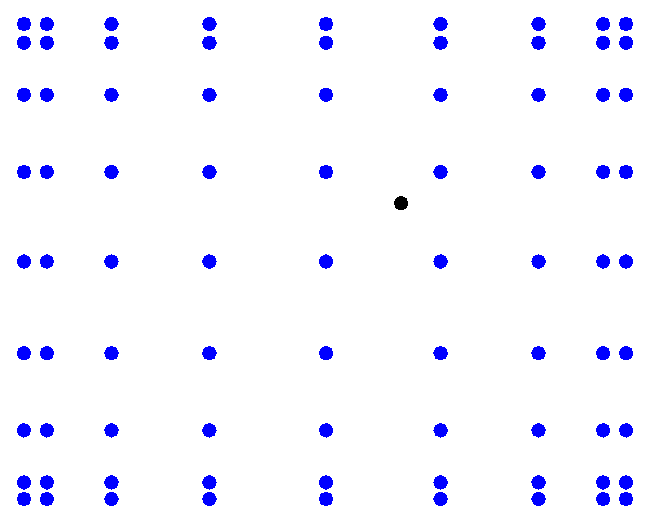
\includegraphics[scale = 0.5]{grid1.eps}
   \label{MERGEB}
 }\hfill
\subfloat[Chebyshev polynomials evaluated along the x-axis at the red points.]{
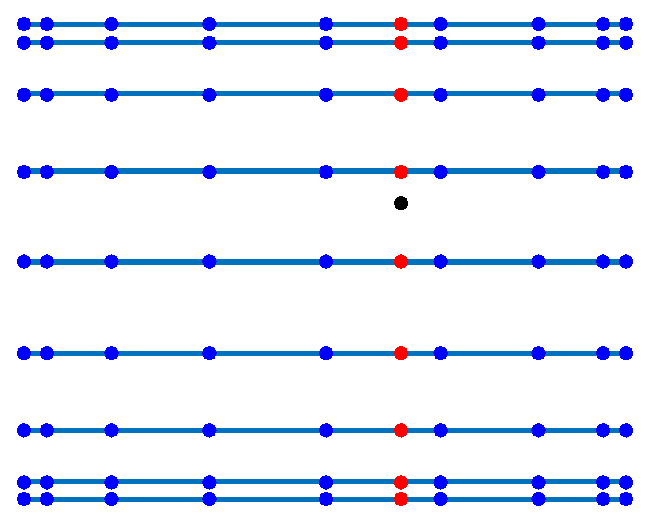
\includegraphics[scale = 0.5]{grid2.eps}
   \label{MERGEA}
 }
 
 \subfloat[Chebyshev polynomial evaluated along at the desired point.]{
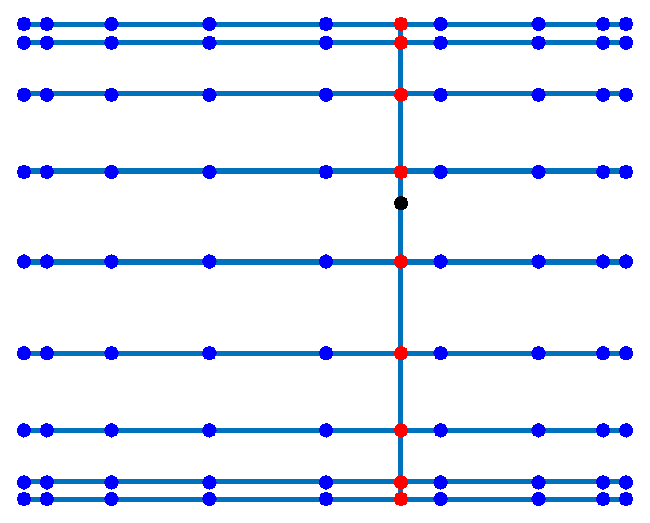
\includegraphics[scale = 0.5]{grid3.eps}
   \label{MERGEA}
 }
\caption{These pictures illustrate how we can computed multivariate Chebyshev interpolants using a one dimensional interpolation method.
}
\label{MULTI_INTERP}
\end{figure}

\section{Some Initial Results}
I have tested the our method on a  2D box with domain $[-1,1]x[-1,1]$. For the function
\begin{equation}
\arctan((x+y)/0.05),
\end{equation}
we have that our method takes 2.135446 seconds (with a splitting tolerance of 1e-14) while Chebfun2 takes 18 seconds.

For the function
\begin{equation}
\arctan(x/0.05)+\arctan(y/0.05),
\end{equation}
our method takes 1.4 seconds while Chebfun2 takes 0.1 seconds. Here is my initial though: Our method's complexity depends on how sharp the features of the function are while Chebfun2's complexity depends on the rank of the function.

\section{RASPEN Solver}
Here I lay out a plan for our to approach the Raspin Solver for a 1D BVP. Here, \bound{0}($\nu$),\bound{1}($\nu$) refer to the left and right interval points of interval($\nu$) as in our paper. The localsolve($\nu$,lbc,rbc) method solves the BVP locally on $\nu$ with the given boundary conditions; this is a method for leaves. The AlternatingSchwartz method would be called on non-leaves. This algorithm can be generalized to higher dimensions, but some care must be given to the boundaries. I will leave this for later.

\begin{algorithm}[!h]
\caption{v=AlternatingSchwartz($\nu$,lbc,rbc)}
\label{alg8}
\begin{algorithmic}
\IF{\child{0}($\nu$) is not a leaf}
\STATE $\hat{\text{rbc}}$ = evalf(\child{1}($\nu$),\bound{1}(\child{0}($\nu$)))
\STATE v0 = AlternatingSchwartz(\child{0}($\nu$),lbc,$\hat{\text{rbc}}$)
\ELSE
\STATE v0 = localsolve(\child{0}($\nu$),lbc,rbc)
\ENDIF

\IF{\child{1}($\nu$) is not a leaf}
\STATE $\hat{\text{lbc}}$ = evalf(\child{0}($\nu$),\bound{0}(\child{1}($\nu$)))
\STATE v1 = AlternatingSchwartz(\child{1}($\nu$),$\hat{\text{lbc}}$,rbc)
\ELSE
\STATE v1 = localsolve(\child{1}($\nu$),lbc,rbc)
\ENDIF
\STATE v = [v0;v1];
\end{algorithmic}
\end{algorithm}

For Algorithm~\ref{alg9}, the residuals of the BVP'S should be included in the nonlinear solve.

\begin{algorithm}[!h]
\caption{c=CourseSolve(T,$x_c$,$D_x$,$D_{xx}$,$u$)}
\label{alg9}
\begin{algorithmic}
\STATE sample(T,$u$)
\STATE [ubglob,udglobdx,uglobd2x] = evalf(T,points(T))
\STATE rglob = ODE(ubglob,udglobdx,uglobd2x)
\STATE $u_c$ = evalf(T,$x_c$)
\STATE $r_c$ = ODE($u_c$,$D_x u_c$, $D_{xx} u_c$)
\STATE sample(T,rglob)
\STATE g = rc + evalf(T,$x_c$)
\STATE c = fsolve(@(s) ODE($s$,$D_x s$,$D_{xx} s$)-g)-$u_c$
\end{algorithmic}
\end{algorithm}

We finally have the RASPEN iteration in \ref{alg10}.
\begin{algorithm}[!h]
\caption{F=Raspen($u$,T,$x_c$,$D_x$,$D_{xx}$,lbc,rbc)}
\label{alg10}
\begin{algorithmic}
\STATE $u_{\text{init}}=u$
\STATE cf=Chebfun(CourseSolve(T,$x_c$,$D_x$,$D_{xx}$,$u$))
\STATE sample(T,u+cf(points(T)))
\STATE Alt = AlternatingSchwartz(T,lbc,rbc)
\STATE sample(T,Alt)
\STATE F = unit-evalf(T,points(T))
\end{algorithmic}
\end{algorithm}

\section{Computing on a Gird}
I completed the code for evaluating the approximation on the grid; this works very fast. The dominate costs for the approximation evaluation on a grid $X$ are:
\begin{itemize}
\item Determining the sub-grids of $X$ are in the nodes of the tree,
\item and calculating the weights.
\end{itemize}
For a tree $T$ with leaves $\{\nu_i\}_{i=1}^N$, let grid($\nu_i$) be the grid of the leaf (in Matlab, this would be stored as a cell array of coordinate vectors). For a forward solver, we would need to evaluate the approximation on $\{\text{grid($\nu_i$)}\}_{i=1}^N$. From what I have seen, a single iteration in the RASPEN solve will require hundreds of evaluations. For the approximation of $tan(x+y)$, the method took 6 seconds to evaluate on the grid.

Looking at the profiler though, almost \%75 to \%80 of the work is determining which points belong to which patches and calculating the weights. These can be pre-calculated. Suppose we have a cell array of the leaves as well as the tree (since I am using the handle class, changes in one data structure will change the other since Matlab uses references).

First, we could use the tree to determine $\text{leafpoints($\nu$)}=\text{points($T$)}\cap\text{domain($\nu$)}$. In this case, $\text{leafpoints($\nu$)}$ could be stored as a cell array of grids. Let's look at an example of a tree in Figure~\ref{Tree_weights} to see how we might precalculate the weights. In this case, the approximate in terms of the leaves is
\begin{equation}
s_{[a,b]}(x) =  w_{\ell_1}(x) s_{[a_{1},b_{1}]}(x) +  w_{r_1}(x)  w_{\ell_2}(x) s_{[a_{21},b_{21}]}(x) + w_{r_1}(x) w_{r_2}(x) s_{[a_{22},b_{22}]}(x)
\end{equation}
In this case we would pre-calculate
\begin{equation}
\begin{aligned}
w_{\ell_1}(x) &\text{ at leafpoints($\nu_1$),} \\
w_{r_1}(x)  w_{\ell_2}(x) &\text{ at leafpoints($\nu_2$),} \\
\text{and } w_{r_1}(x) w_{r_2}(x)  &\text{ at leafpoints($\nu_3$).}
\end{aligned}
\end{equation}

For a general tree, we can write a recursive function to do this as seen in Algorithm~\ref{alg11}. For a node $\nu$, let $\text{weight($\nu$)}$ be the weight multiplied by the approximate for the node (i.e., in Figure~\ref{Tree_weights} $\text{weight($\nu_1$)}=w_{\ell_2}(x)$). For the root of the tree, we set the weight to the constant function 1. In my code I use a standard weight with parameters to shift and scale; this implies that we can just store the parameters for the weight used at the node of the tree. For each leaf $\nu_i$ of the tree $T$, we set
\begin{equation}
\text{weightvals($\nu_i$)=CalculateWeights(root($T$),domain($\nu_i$),leafpoints($\nu_i$))}.
\end{equation}
Let leafpointindex($\nu_i$) be the indices of the points in leafpoints(root($T$)). I describe in Algorithm~\ref{alg12} how to evaluate the approximation on the grids of the tree. This can easily be implemented using a parfor loop if needed.

\begin{algorithm}[!h]
\caption{w=CalculateWeights($\nu$,dom,$X$)}
\label{alg11}
\begin{algorithmic}
\IF{$\nu$ is a leaf}
\STATE $\text{w} \leftarrow \left . \text{weights($\nu$)} \right |_{X}$
\ELSIF{$\text{dom}\subseteq \text{domain(\child{0}($\nu$))}$}
\STATE $\text{w} \leftarrow \left . \text{weights($\nu$)} \right |_{X}.*\text{CalculateWeights(\child{0}($\nu$),dom,$X$)}$
\ELSE
\STATE $\text{w} \leftarrow \left . \text{weights($\nu$)} \right |_{X}.*\text{CalculateWeights(\child{1}($\nu$),dom,$X$)}$
\ENDIF
\end{algorithmic}
\end{algorithm}



\begin{algorithm}[!h]
\caption{F=evalfTreeGrid($T$)}
\label{alg12}
\begin{algorithmic}
\FOR{ each leaf $\nu_i$ of $T$}
\STATE $F_i = \text{zeros}(\text{length}(T),1)$
\STATE $F_i(\text{leafpointindex($\nu_i$)}) \leftarrow \text{weightvals($\nu_i$)}.*\text{evalf}(\nu_i,\text{leafpoints($\nu_i$)})$
\ENDFOR
\STATE $F = \sum_{i=1}^N F_i$.
\end{algorithmic}
\end{algorithm}

\begin{figure}
\centering
     \begin{forest}
for tree={circle,draw, l sep=20pt,,scale=0.98}
[ {$\begin{array}{c}
[a,b] \\
s_{[a,b]}(x)
\end{array}$}
    [ {$\begin{array}{c}
 [a_1,b_1]  \\
s_{[a_{1},b_{1}]}(x) \\
 w_{\ell_1}(x) \\
 \nu_1
\end{array}$},name=left_p]
    [ {{$\begin{array}{c}
    [a_2,b_2] \\
s_{[a_{2},b_{2}]}(x) \\
 w_{r_1}(x) 
\end{array}$}} 
      [{$\begin{array}{c}
 [a_{21},b_{21}] \\     
s_{[a_{21},b_{21}]}(x) \\
 w_{\ell_2}(x) \\
 \nu_2
\end{array}$},name=right_p] 
      [{$\begin{array}{c}
  [a_{22},b_{22}] \\    
s_{[a_{22},b_{22}]}(x) \\
 w_{r_2}(x) \\
  \nu_3
\end{array}$}] 
  ] 
]
]
\end{forest}
\caption{An example of a simple tree with nodes ${\nu_1,\nu_2,\nu_3}$, where each node is labeled with its domain, PU approximate and weight (in that order).}
\label{Tree_weights}
\end{figure}

\section{Over determined least squares method}
Suppose we have an orthogonal set of tensor product chebyshev polynomials $\{ T_k(x,y) \}_{k=1}^{\infty}$ for $[-1,1]\times[-1,1]$ (i.e. the set of polynomials is formed from the tensor product of the polynomials in $x$ and $y$). Our goal is to approximate the function $f:\Omega \to \R$, with $\Omega \subset [-1,1]\times[-1,1]$. Let
\begin{align}
G_N = \text{span}\{T_k(x,y):k<N\}
\end{align}
and
\begin{align}
g_N = \argmin_{g \in G_N} \| g(x,y)-f(x,y) \|_{L^2(\Omega)}.
\end{align}
The first question we might answer is: Does $g_N \to f$ in the $L^2(\Omega)$ norm? I would think so. If there exists an extension $\varepsilon f(x,y):[-1,1]\times[-1,1] \to \R$ such that $\varepsilon f(x,y) \equiv f(x,y)$ on $\Omega$, then a straight forward convergence argument can be made. I would need to read more about this though.

Though we might could find an exact representation for $g_N$, it will either be
\begin{itemize}
\item cumbersome to compute (we would likely need to compute integrals over $\Omega$),
\item unstable to compute (as seen in the Fourier extensions).
\end{itemize}

Let $X_M \subset \Omega$ be a discrete set of $M$ points. We instead solve for

\begin{align}
\hat{g}_N = \argmin_{g \in G_N} \| \left . (g-f) \right |_{X_M} \|_2
\end{align}

The first question that comes to mind is: as $M \to \infty$, does $\hat{g}_N \to g_n$ (at least in exact arithmetic)? I would suspect so.

\subsection{Simple 2D experiment}

As a simple experiment, I try to approximate
\begin{align}
f(x,y) = \cos((x-1)^2+(y-1)^2)
\end{align}
In the region
\begin{align}
\Omega = \{(x,y) \in [-1,1] \times [-1,1]: (Ax+By+C)/B \geq 0 \}
\label{trig_region}
\end{align}
i.e. the region in $[-1,1] \times [-1,1]$ above the line $Ax+By+C=0$. As a first test, I set $A=B=1$, and look at regions for $C \in [0,2]$. For $C=0$, this gives the half the square along its diagonal and $C=2$ gives the whole square. Figure~\ref{region_c} shows the region with $C=1.2$.
\begin{figure}[!h]
\centering
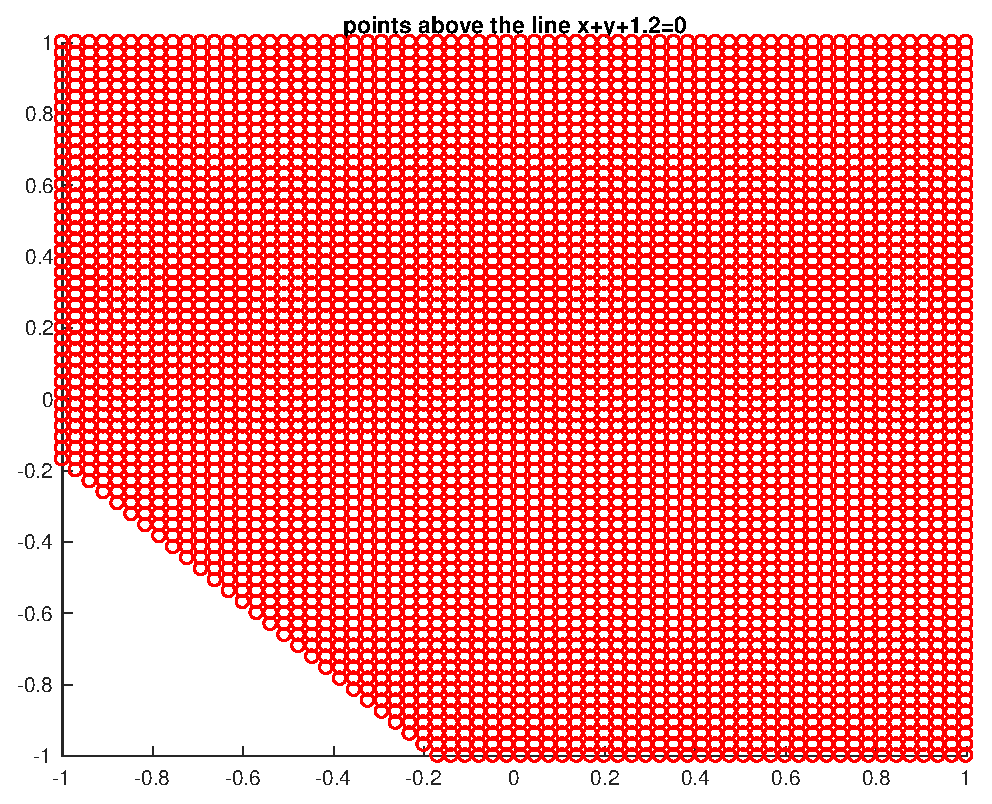
\includegraphics[scale = 0.5]{subset_plot.eps}
\caption{Region with $A=B=1$, $C=1.2$.}
\label{region_c}
\end{figure}

For this problem, I let
\begin{align}
G_N = \text{span}\{T_i(x) T_j(y):i,j \leq N\}
\end{align}
where $T_i(x)$ is the $i_{th}$ Chebyshev polynomial and
\begin{align}
\hat{g}_N = \argmin_{g \in G_N} \| \left . (g-f) \right |_{X} \|_2
\end{align}
for a discrete set $X \in \Omega$. For my test, I set $N=33$, and find $\hat{g}_N$ when
\begin{itemize}
\item $X$ is the subset of the $66 \times 66$ equidistant points in $\Omega$,
\item $X$ is the subset of the $66 \times 66$ Chebyshev points (i.e. a tensor product) in $\Omega$,
\item and $X$ is the subset of the $66 \times 66$ Chebyshev points in $\Omega$ with 66 equidistant points added to the diagonal boundary.
\end{itemize}
To measure the accuracy of $\hat{g}_N $ as approximation, we compute the inf norm for the $132 \times 132$ equidistant points in $\Omega$. The results can be seen in Figure~\ref{line_err_plots}. It would seem:
\begin{itemize}
\item If there is less empty space the error is lower,
\item we are better off using Chebyshev points instead of equidistant points,
\item and there is a benefit to adding points along the boundary.
\end{itemize}


\begin{figure}[!h]
\centering
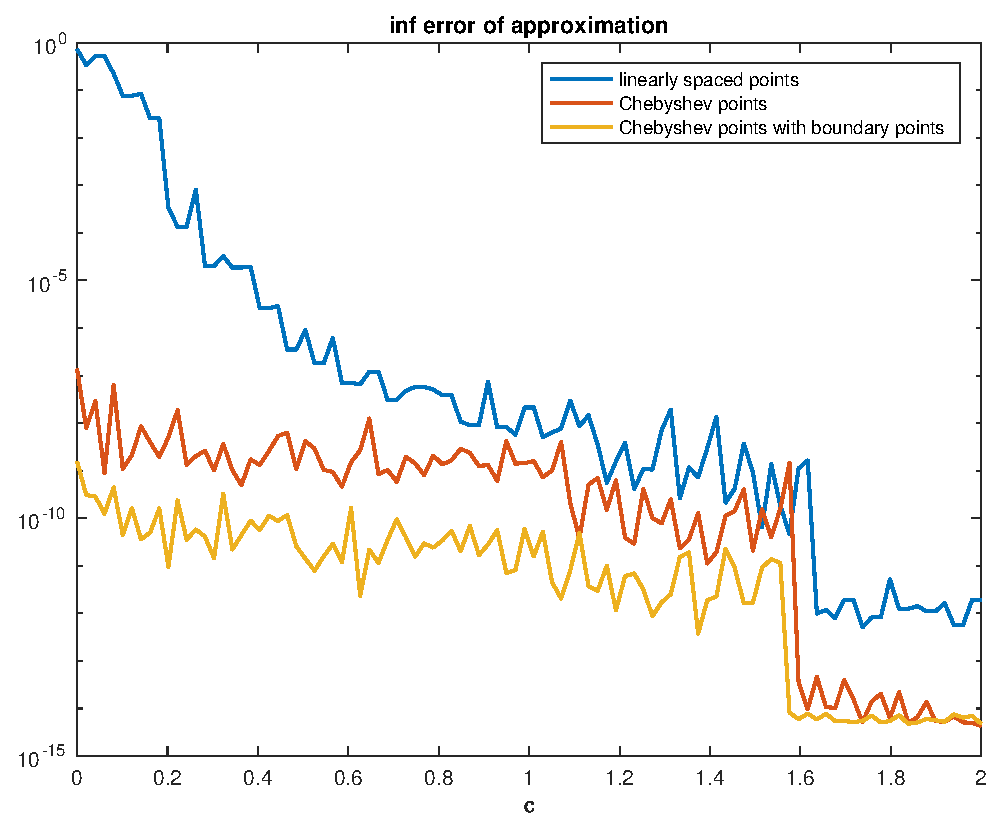
\includegraphics[scale = 0.5]{line_err_plot.eps}
\caption{Semi-log plot of inf error for $C \in [0,2]$.}
\label{line_err_plots}
\end{figure}

For a second test, we set
\begin{align}
\Omega = [-1,1] \times [-1,1] \cap B_{4}([c,0])
\label{circ_region}
\end{align}
for $c \in [3,4.5]$. Figure~\ref{region_circ} shows the region with $c=3.5$. We test with for similar collocation points as before, but included linearly spaced points with points added to the boundary. The results can be seen in Figure~\ref{circ_err_plots}. Here we see that Chebyshev points with the boundary gives the best results.

\begin{figure}[!h]
\centering
\includegraphics[scale = 0.25]{circ_region.png}
\caption{Region with $c=3.5$.}
\label{region_circ}
\end{figure}

\begin{figure}[!h]
\centering
\includegraphics[scale = 0.5]{circ_error.eps}
\caption{Semi-log plot of inf error for $C \in [0,2]$.}
\label{circ_err_plots}
\end{figure}

\section{Over determined least squares method with rank deficient matrices}

When we  use a collocation matrix $A \in \C^{m \times n}$ for a subset $\Omega$ on the square $[-1,1] \times [-1,1]$ we often find that $A$ is rank deficient. This is unsurprising since we are not specifying function values outside of $\Omega$. Suppose that $A$ has rank $r$. Then $A$ has a QR decomposition where
\begin{align}
R = \begin{pmatrix}
 R_{11} & R_{12} \\
 0 & 0
 \end{pmatrix}
 \begin{array}{l}
 \} r \\
 \} n-r
 \end{array}
\end{align}
 with $R_{11}$ nonsingular. In this case
 \begin{align}
 \argmin_{x \in \C^n} \left \| Ax-b\right \|_2
 \end{align}
will have multiple solutions. Let
\begin{align}
M = \left \{ x |  \argmin_{x \in \C^n} \left \| Ax-b\right \|_2 \right \}
\end{align}
i.e. the set of $x$ that minimizes the least squares problem. We can find a unique solution if try to find $x$ that satisfies
\begin{align}
\argmin_{x \in M} \| B x \|_2
\label{cool_prob}
\end{align}
where $B$ has linearly independent rows. For this problem $x$ has the form
\begin{align}
x = \begin{pmatrix}
 x_1 \\
 x_2
 \end{pmatrix}
\end{align}
where $x_2$ is a free parameter and 
\begin{align}
x_1 = R_{11}^{-1}(Q_1^{T}b-R_{12}x_2).
\end{align}
Let $S$ be the matrix such that
\begin{equation}
R_{11} S = R_{12}.
\end{equation}
In order to solve (\ref{cool_prob}), we set
\begin{equation}
x_2 = \argmin_{\hat{x}_2}\left \| B \begin{pmatrix} S \\ -I_{n-r} \end{pmatrix} \hat{x}_2 - B \begin{pmatrix} R_{11}^{-1}Q_1^{T}b \\ 0 \end{pmatrix}
\right \|_2.
\end{equation}
The solution return by $x=A\backslash b$ in Matlab is the \textbf{basic solution}, where $x_1$ is found by setting $x_2=0$.

We repeat the experiments we did before on both sets of domains, where we record the errors for:
\begin{itemize}
\item $B=I$ (in this case we minimize the norm of the coefficients),
\item $B=D_x+D_y$, where $D_x$, $D_y$ are the differentiation matrices for the coefficients (in this case we minimize the norm of the coefficients of the divergence)
\item $B=D_x^2+D_y^2$ (in this case we minimize the norm of the coefficients of the laplacian),
\item and the coefficients returned by the basic solution. 
\end{itemize}

For the region with the triangle cut off defined in (\ref{trig_region}), we record the errors for the function
\begin{align}
f(x,y) = \cos((x-1)^2+(y-1)^2)
\end{align}
and its derivative for $C \in [0,1.5]$; for $C$ higher than $1.5$ the collocation matrix has full rank, making each of the different cases the same. For this experiment we used Chebyshev points with points added at the boundary. I repeat this experiment for the circular defined in (\ref{circ_region}) for $C \in [3.3 , 4.5]$.

\begin{figure}[!htb]
\centering
\subfloat[]{
\includegraphics[scale = 0.3]{err_plots_rd_line_c.eps}
   \label{lineplotda}
 }\hfill
\subfloat[]{
\includegraphics[scale = 0.3]{err_plots_diff_rd_line_c.eps}
   \label{lineplotdb}
 }
\label{lineplotd}
\caption{Infinity errors for the region defined in  defined in (\ref{trig_region}) for $C \in [0,1.5]$.}
\end{figure}

\begin{figure}[!htb]
\centering
\subfloat[]{
\includegraphics[scale = 0.3]{err_plots_rd_circ_c.eps}
   \label{circplota}
 }\hfill
\subfloat[]{
\includegraphics[scale = 0.3]{err_plots_diff_rd_circ_c.eps}
   \label{circplotb}
 }
\label{circplot}
\caption{Infinity errors for the region defined in  defined in (\ref{circ_region}) for $C \in [3.3,4.5]$.}
\end{figure}

\begin{figure}[!htb]
\centering
\subfloat[]{
\includegraphics[scale = 0.3]{err_plots_rd_line_lin.eps}
   \label{lineplotlda}
 }\hfill
\subfloat[]{
\includegraphics[scale = 0.3]{err_plots_diff_rd_line_lin.eps}
   \label{lineplotldb}
 }
\label{lineplotl}
\caption{Infinity errors for the region defined in  defined in (\ref{trig_region}) for $C \in [0,1.5]$ using linearly spaced points.}
\end{figure}

\begin{figure}[!htb]
\centering
\subfloat[]{
\includegraphics[scale = 0.3]{err_plots_rd_circ_lin.eps}
   \label{circplotla}
 }\hfill
\subfloat[]{
\includegraphics[scale = 0.3]{err_plots_diff_rd_circ_lin.eps}
   \label{circplotlb}
 }
\label{circplotl}
\caption{Infinity errors for the region defined in  defined in (\ref{circ_region}) for $C \in [3.3,4.5]$ using linearly spaced points.}
\end{figure}

\section{Partition of Unity geometric refinement}

Suppose we have a domain $\Omega \in \R^2$ which is not a rectangle, and function $f(x):\Omega \to \R$. Our goal is to create an adaptive method by overlaying $\Omega$ with overlapping squares. We first start by finding a square $[a,b] \times [c,d]$ such that $\Omega \subseteq [a,b] \times [c,d]$. For the adaptive refinement, we use the method we have for the square. We refine by splitting the square along a certain dimension, and recursively repeat this until we have an accurate PU approximation. The PU weights have support on the squares, while the approximations are only defined in the domain itself.

In this case each leaf of the tree is a rectangle. For a leaf $\nu$ if $\Omega \cap \text{domain}(\nu) \neq \text{domain}(\nu)$ (i.e. $\Omega \cap \text{domain}(\nu)$ is not square) we use the least square method; otherwise we use the standard Chebyshev method. We define a LSPATCH2D object which is a leafPatch object in Section~\ref{Structsec} with the following added properties:
\begin{itemize}
\item BoxDomain($\nu$):the domain of the outer box domain.
\item MaxLengths($\nu$):array of maximum lengths of for BoxDomain($\nu$).
\item InteriorPoints($\nu$): the set of test points as seen in Figure~\ref{Split_patch_single}.

\end{itemize}
For these leaves, $\text{domain}(\nu) = \Omega \cap \text{BoxDomain}(\nu)$. We add an additional method:
\begin{itemize}
\item IsGeometricallyRefined($\nu$):determines if refinement is needed based on the geometry of $\Omega$.
\end{itemize}
The method can be seen in Algorithm~\ref{alg12}. The goal is to have a patch structure that follows the geometry of $\Omega$.


The first challenge for this method is to determine when to drop leaves based on the geometry of $\Omega$. For instance, suppose we split the leaf $\nu$ as seen in Figure~\ref{Split_patch_1}. In this case, the child $\nu_0$ becomes unnecessary since the domain sits entirely in $\text{BoxDomain}(\nu_1)$. For a tree $T$, we drop $\nu_0$ be replacing $\nu$ with $\nu_1$. The splitting algorithm can be seen in Algorithm~\ref{alg13}. Examples of the geometric refinement can be seen in Figure~\ref{geometric_refine}.

\begin{figure}[!h]
\centering
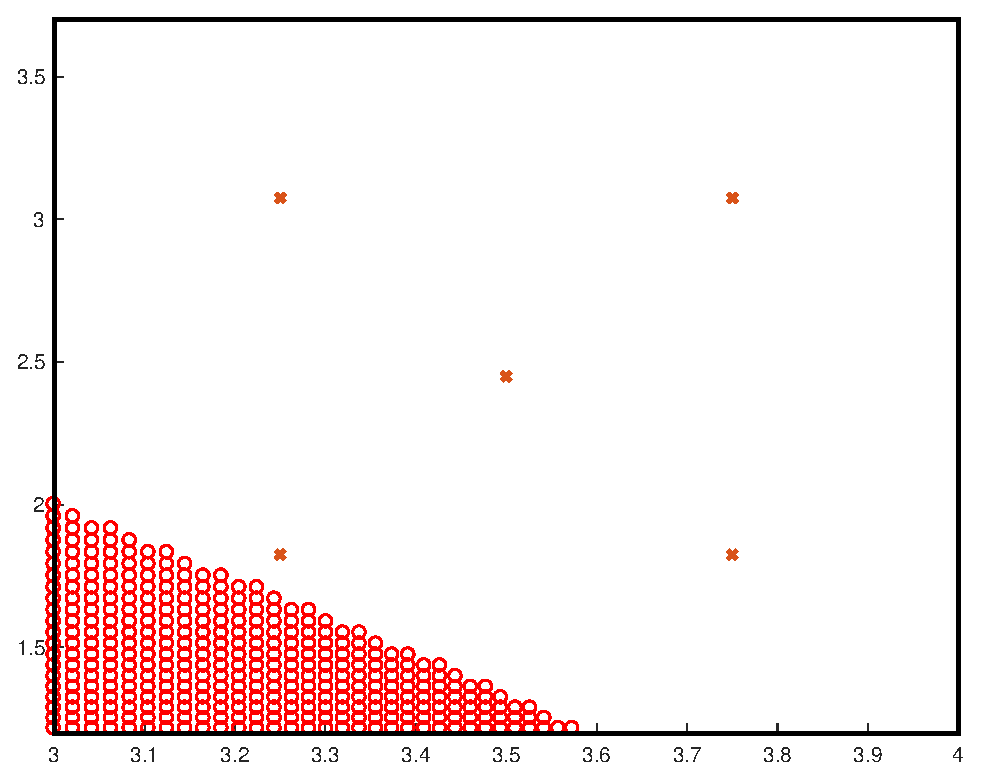
\includegraphics[scale = 0.5]{single_patch_cosine.eps}
\caption{An example of a splitting where a patch $\nu$ would be geometrically refined. Here the red circles indicate the domain $\Omega$, and the x's are the points InteriorPoints($\nu$).}
\label{Split_patch_single}
\end{figure}

\begin{figure}[!h]
\centering
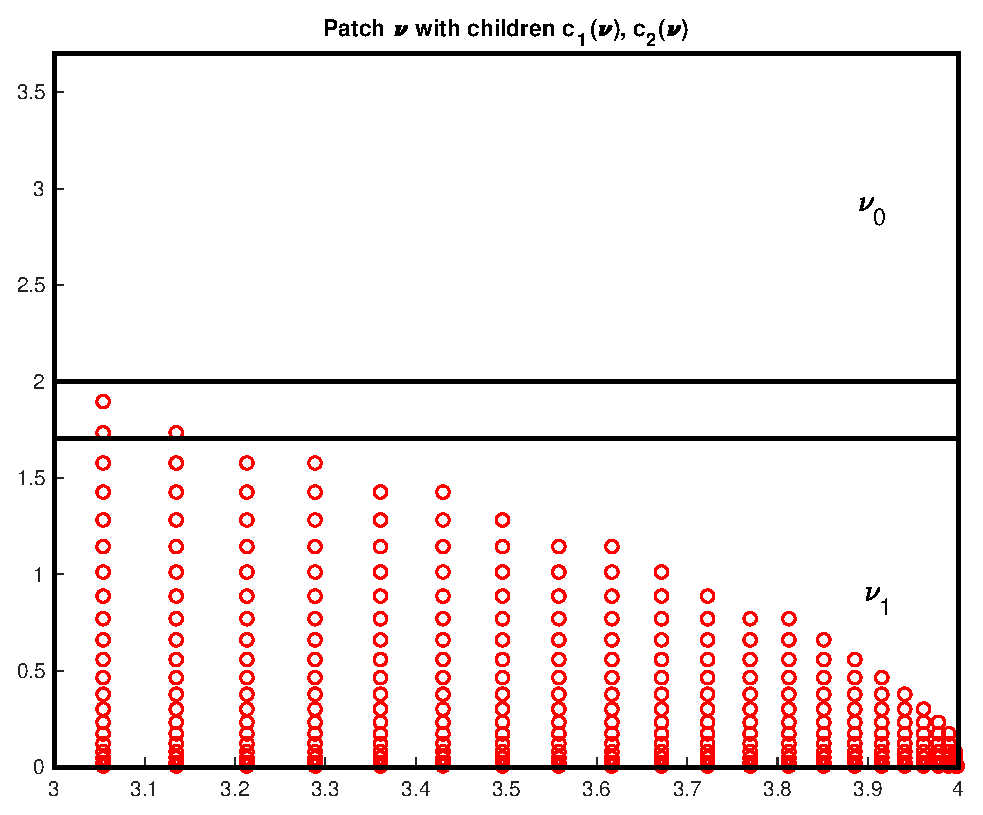
\includegraphics[scale = 0.5]{split_patch_cosine.eps}
\caption{An example of a patch $\nu$ and domain $\Omega$ where the InteriorPoints($\nu$) do not lie in $\Omega$.}
\label{Split_patch_1}
\end{figure}



\begin{algorithm}[!h]
\caption{T = IsGeometricallyRefined($\nu$)}
\label{alg12}
\begin{algorithmic}
\IF{The lengths of BoxDomain($\nu$) are less than MaxLengths($\nu$) \textbf{and} at least one point from InteriorPoints($\nu$) lies in domain($\nu$)}
\STATE $\nu$ is geometrically refined.
\ELSE
\STATE $\nu$ is not geometrically refined.
\ENDIF
\end{algorithmic}
\end{algorithm}

\begin{algorithm}[!h]
\caption{Child = SplitLeaf($\nu$,$f(x)$) (method for LSPATCH2D)}
\label{alg13}
\begin{algorithmic}
\IF{$\nu$ is geometrically refined \textbf{and} $\nu$ can refine $f(x)$ on domain($\nu$)}
\STATE Child = $\nu$
\ELSE
\STATE{Define domain0 and domain1 as the domains of the rectangular patches split along the dimension of greatest length of BoxDomain($\nu$).}
 \FOR{k=0,1} 
 \IF{If $\text{domaink} \cap \Omega= \text{domaink}$}
 \STATE $\nu_k$:= ChebPatch with domaink
 \ELSE 
 \STATE $\nu_k$:= LSPATCH2D with domaink
 \ENDIF 
 \ENDFOR
 \IF{If domain($\nu$) $\subseteq$ domain(\child{0}($\nu$))}
 \STATE Child = $\nu_0$
 \ELSIF{If domain($\nu$) $\subseteq$ domain(\child{1}($\nu$))}
  \STATE Child = $\nu_1$
 \ELSE
 \STATE Child = A PUPatch with children \child{0}(Child)=$\nu_0$,\child{1}(Child):=$\nu_1$
\ENDIF
\ENDIF
\end{algorithmic}
\end{algorithm}

\begin{figure}[!htb]
\centering
\subfloat[]{
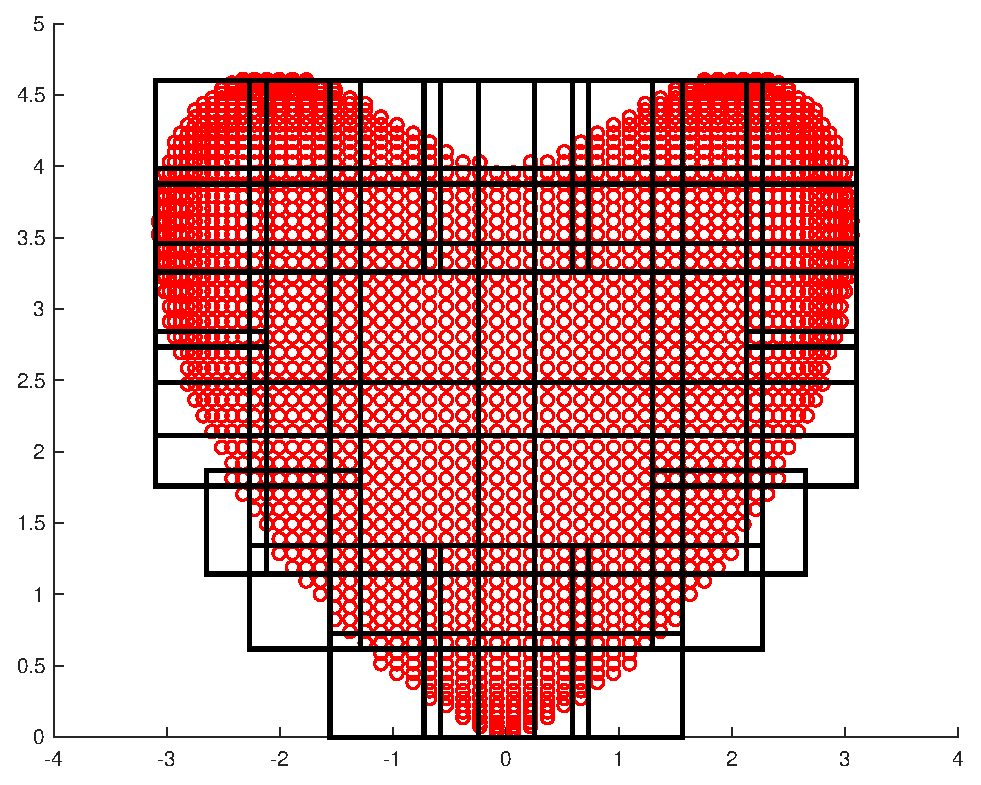
\includegraphics[scale = 0.3]{heart_plot.eps}
   \label{geoma}
 }\hfill
\subfloat[]{
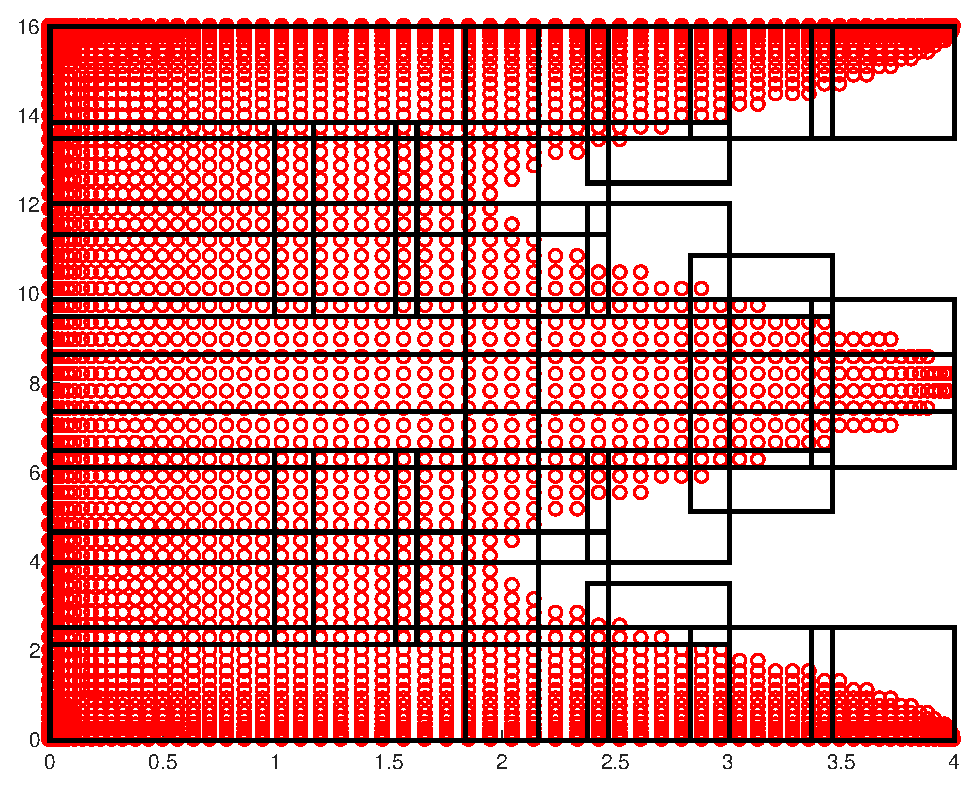
\includegraphics[scale = 0.3]{consine_plot.eps}
   \label{geomb}
 }
\caption{An example of a geometric refinement for (a) a heart and (b) a domain whose right boundary is dictated by a cosine curve.}
\label{geometric_refine}
\end{figure}

\subsection{Some comments and questions}
\begin{itemize}
\item I am not attached to the way this algorithm is implemented right now, and believe it can be improved upon. I am thinking that if at least three of the interior points of $\nu$ are in $\Omega$, we mark the patch as geometrically refined regardless of the size of the outer box.
\item We could resize the outerbox of the leaves before we split. While this does avoid the problem of dropping leaves, I don't think implementation will be less complicated than now. The only way I know how to resize the outerbox is to sample the domain and fit a box around that.
\end{itemize}

\section{Kronecker products and vec in 3D}
For two dimensional arrays, we have the well known result
\begin{equation}
\vecm(ACB) = (B^T \otimes A) \vecm (C).
\label{kronvec}
\end{equation}
This can be useful for forming matrices for 2D tensor product approximations. For instance, suppose that we have a Chebyshev tensor product approximation
\begin{equation}
s(x,y) = \sum_{i=1}^{N_x} \sum_{j=1}^{N_y} c_{ij} T_i(x)T_j(y),
\end{equation}
along with points $\{x_n\}_{n=1}^{S_x}$, $\{y_n\}_{n=1}^{S_y}$ that we wish to approximate $s(x,y)$ given any set of coefficients $(c_{i,j})$. Define a matrix $M^x$ such that
\begin{equation}
\begin{aligned}
	M_{i,j}^x &= T_j(x_i).
\end{aligned}
\end{equation}
Given a vector of coefficients $d = [d_1,\dots,d_{N_x}]^T \in \C^{N_x}$ we have
\begin{equation}
(M^x d)_n = \sum_{i=1}^{N_x} d_n T_j(x_n),
\end{equation}
i.e. $M^x$ will evaluate a Chebyshev approximation at $\{x_n\}_{n=1}^{S_x}$ given a vector of coefficients. We can similarly define a matrix $M^y$ for points $\{y_n\}_{n=1}^{S_y}$. Define $A \in \C^{S_x S_y}$ such that
\begin{equation}
A_{nm} = \sum_{i=1}^{N_x} \sum_{j=1}^{N_y} c_{ij} T_i(x_n)T_j(y_m).
\end{equation}
Using our matrices $M^x$ and $M^y$ we can deduce that
\begin{equation}
\begin{aligned}
A_{nm} &= \sum_{i=1}^{N_x} \sum_{j=1}^{N_y} M_{ni}^x c_{ij} M_{mj}^y \\
       &= \sum_{i=1}^{N_x} M_{ni}^x \sum_{j=1}^{N_y} c_{ij} (M^y)_{jm}^T \\
       &= \sum_{i=1}^{N_x} M_{ni}^x ((c_{ij}) (M^y)^T)_{im} \\
       &=  (M^x(c_{ij}) (M^y)^T)_{nm}.
\end{aligned}
\end{equation}
We thus have from (\ref{kronvec}) that
\begin{equation}
	\vecm(A) = (M^y \otimes M^x) \vecm((c_{ij})).
	\label{2DKron}
\end{equation}
Suppose now we want to do the same but for the approximation 
\begin{equation}
s(x,y,z) = \sum_{i=1}^{N_x} \sum_{j=1}^{N_y} \sum_{k=1}^{N_z} c_{ijk} T_i(x)T_j(y)T_k(z),
\end{equation}
where we also have points $\{z_n\}_{n=1}^{S_z}$ and interpolation matrix $M^{z}$. Suppose we have a set of coefficients $C \in \C^{N_x N_y N_z}$. In MATLAB,
\begin{equation}
\vecm(C) = 
\begin{bmatrix}
\vecm(C(:,:,1))	\\
\vecm(C(:,:,2))	\\
\vdots \\
\vecm(C(:,:,N_z))
\end{bmatrix}.
\end{equation}
Now define $A \in \C^{S_x S_y S_z}$ such that
\begin{equation}
A_{nmp} = \sum_{i=1}^{N_x} \sum_{j=1}^{N_y}  \sum_{k=1}^{N_z}  C_{ijk} T_i(x_n)T_j(y_m)T_k(y_p).
\end{equation}
We first have
\begin{equation}
	\begin{aligned}
		A(:,:,p)_{nm} &= \sum_{i=1}^{N_x} \sum_{j=1}^{N_y}  \sum_{k=1}^{N_z} C_{ijk} M_{ni}^x M_{mj}^y M_{pk}^z \\
		 		 &= \sum_{k=1}^{N_z} M_{pk}^z  \sum_{i=1}^{N_x} \sum_{j=1}^{N_y} C_{ijk} M_{ni}^x M_{mj}^y \\
		 		 &= \sum_{k=1}^{N_z} M_{pk}^z (M^x C(:,:,k) (M^y)^T)_{nm}.
	\end{aligned}
\end{equation}
Thus from (\ref{2DKron}) we can infer that
\begin{equation}
\vecm(A(:,:,p)) = \sum_{k=1}^{N_z} M_{pk}^z (M^y \otimes M^x) \vecm(C(:,:,k))
\end{equation}
and can further argure that
\begin{equation}
	\begin{aligned}
		& \sum_{k=1}^{N_z} M_{pk}^z (M^y \otimes M^x) \vecm(C(:,:,k)) \\
		&= [M_{p1}^z (M^y \otimes M^x) \dots M_{p N_z}^z (M^y \otimes M^x)] \begin{bmatrix}
			\vecm(C(:,:,1)) \\
			\vdots \\
			\vecm(C(:,:,N_z))
		\end{bmatrix} \\
		&= (M^z(p,:) \otimes (M^y \otimes M^x)) \vecm(C)	,
	\end{aligned}
\end{equation}
given how MATLAB vectorizes multidimensional arrays. We thus have
\begin{equation}
\begin{aligned}
	\vecm(A) = \begin{bmatrix}
		M^z(1,:) \otimes (M^y \otimes M^x) \\
		\vdots \\
		M^z(N_z,:) \otimes ( M^y \otimes M^x) 
	\end{bmatrix} \vecm(C)
\end{aligned}
\end{equation}
giving us
\begin{equation}
	\vecm(A) = (M^z \otimes M^y \otimes M^x) \vecm(C).
\end{equation}

\section{PU derivatives again}
Suppose we have intervals $[0,t]$, $[-t,0]$ and we approximate the function $f(x)$ with
\begin{equation}
s(x) = w_{\ell}(x)s_{\ell}(x) +w_{r}(x)s_{r}(x)	
\end{equation}
where $\{w_{\ell}(x),w_{r}(x)\}$ forms a PU with $\{[0,t],[-t,0]\}$ and $s_{\ell}(x),s_{r}(x)$ approximate $f(x)$ on the respective intervals. 
In our first PU paper in (15) we found
\begin{equation}
\begin{aligned}
\left | f'(x)-s'(x) \right | &\leq \left | w_{\ell}(x) \lp f'(x)-s_{\ell}'(x) \rp \right |+\left | w_{r}(x) \lp f'(x)-s_{r}'(x) \rp \right | \\
&+\left | w_{\ell
}'(x) \lp f(x)-s_{\ell}(x) \rp \right | +\left | w_{r}'(x) \lp f(x)-s_{r}(x) \rp \right |,
\end{aligned}
\end{equation}
implying
\begin{equation}
\begin{aligned}
\left \| f'(x)-s'(x) \right \|_{L_{\infty}[-1,1]} \leq \max \lp \left \| f'(x)-s_{\ell}'(x) \right \|_{L_{\infty}[-1,t]} , \left \| f'(x)-s_{r}'(x) \right \|_{L_{\infty}[-t,1]} \rp & \\
+\left \| w_{\ell}'(x) \right \|_{L_{\infty}[-t,t]} \max \lp \left \| f(x)-s_{\ell}(x)\right \|_{L_{\infty}[-t,t]}
, \left \| f(x)-s_{r}(x)\right \|_{L_{\infty}[-t,t]} \rp. &
\end{aligned}
\label{diff_error_2}
\end{equation}
and chose the overlap by balancing the two terms in (\ref{diff_error_2}). While examining the Shepard's weights, I found that the derivatives can get quite complicated. My hypothesis is that if we have sufficient overlap that
\begin{equation}
w_{\ell}(x)s_{\ell}'(x)+w_{r}(x)s_{r}'(x)	
\end{equation}
can sufficiently approximate $f'(x)$.

 We have
\begin{equation}
s'(x) = w_{\ell}(x)s_{\ell}'(x) + w_{r}(x)s_{r}'(x) + w_{\ell}'(x)s_{\ell}(x) + w_{r}(x)s_{r}(x).
\end{equation}
Since $w_{\ell}+w_{r}=1$, we have $w_{\ell}'+w_{r}'=0$. Thus
\begin{equation}
s'(x) = w_{\ell}(x)s_{\ell}'(x) + w_{r}(x)s_{r}'(x) + w_{\ell}'(x)(s_{\ell}(x)-f(x)) + w_{r}(x)(s_{r}(x)-f(x)).
\end{equation}
We can thus infer
\begin{equation}
\begin{aligned}
& s'(x) - f'(x)  \\
& - w_{\ell}'(x)(s_{\ell}(x)-f(x)) - w_{r}(x)(s_{r}(x)-f(x))   \\ &=w_{\ell}(x)s_{\ell}'(x) + w_{r}(x)s_{r}'(x) - f'(x).	
\end{aligned}
\end{equation}
Letting
\begin{equation}
\hat{s}(x) = w_{\ell}(x)s_{\ell}'(x) + w_{r}(x)s_{r}'(x),
\end{equation}
we get
\begin{equation}
\begin{aligned}
\| \hat{s}(x) - f(x) \| \leq &\|s'(x)-f'(x) \| + \\ & \left \| w_{\ell}'(x) \right \|_{L_{\infty}[-t,t]} \max \lp \left \| f(x)-s_{\ell}(x)\right \|_{L_{\infty}[-t,t]}
, \left \| f(x)-s_{r}(x)\right \|_{L_{\infty}[-t,t]} \rp.	
\end{aligned}
\end{equation}
We can infer from here that $\hat{s}(x)$ can approximate $f'(x)$.

\section{Chebyshev tensor product approximation}

\subsection{Chebyshev interpolation}
\label{sec_cheb}
We use Chebyshev interpolants for our partition of unity method because they enjoy spectral convergence. Suppose that $f(x)$ is analytic inside a  Bernstein ellipse $E_\rho$ (an ellipse with foci $\pm 1$ and semi-major axis $\rho>1$). We then have Theorem 6 from \cite{trefethen2000spectral}:
\begin{theorem} Suppose $f(z)$ is analytic on and inside the Bernstein ellipse $E_\rho$. Let $p_n$ be the polynomial that interpolates $f(z)$ at $n+1$ Chebyshev points of the second kind. Then there exists a constant $C>0$ such that for all $n>0$,
$$ \left \| f(x)-p_n(x) \right \|_{\infty} \leq C  \rho^{-n}.$$
 \end{theorem}
If $f(x)$ is Lipschitz continuous on $[-1,1]$ then
\begin{equation}
f(x) = \sum_{k=0}^\infty a_k T_k(x), \quad a_k = \frac{2}{\pi} \int_{-1}^1 \frac{f(x) T_k(x)}{\sqrt{1-x^2}} dx,
\end{equation}
where $T_k$ denotes the degree $k$ Chebyshev polynomial (and for $a_0$, we multiply by $\frac{1}{\pi}$ instead of $\frac{2}{\pi}$). Furthermore if $p_n(x)$ is the $n$th degree Chebyshev interpolant then
\begin{equation}
f(x)-p_n(x) = \sum_{k=n+1}^{\infty} a_k \lp T_k(x)-T_m(x)\rp,
\end{equation}
where
\begin{equation}
m = \left [ (k+n-1)(\text{mod }2n) - (n-1)\right ],
\end{equation}
implying we can determine the accuracy of the interpolant $p_n(x)$ by inspecting the Chebyshev coefficients \cite{Trefethen2013}. Chebfun's standardChop method determines the minimum required degree by searching for a plateau of low magnitude coefficients \cite{Aurentz:2017:CCS:3034774.2998442}.  For example, Figure~\ref{Coeff_example} shows the first 128 coefficients of $f(x)=\exp \lp \sin \lp \pi x \rp \rp$. We see that all coefficients after the first 46 have magnitude less than $10^{-15}$. In this case, Chebfun determines the ideal degree to be 50.
\begin{figure}[!htb]
\centering
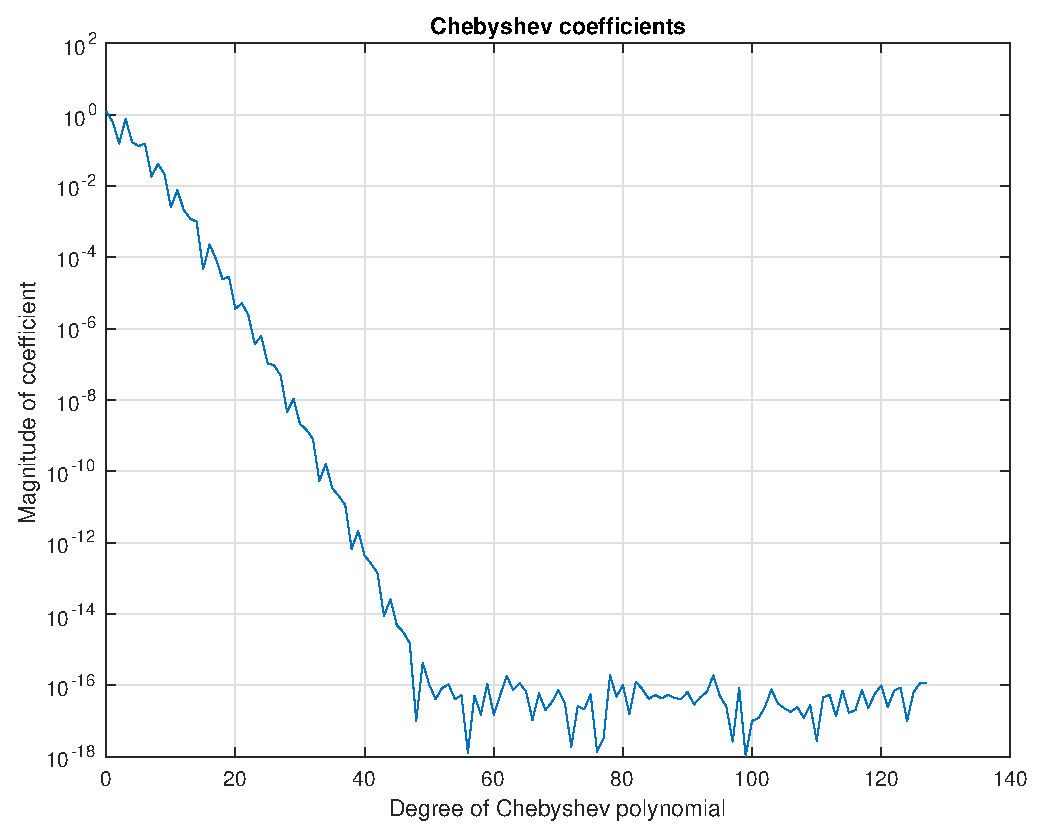
\includegraphics[scale = 0.5]{../tear-films-numerical-pde/1dPOU/PU_PAPER/coeff_plot.eps}
\caption{Chebyshev coefficients for $f(x)=\exp \lp \sin \lp \pi x \rp \rp$.}
\label{Coeff_example}
\end{figure}

Suppose now we are approximation $f(\vect{x}) \in [-1,1]^n \to \C$. For a multivariate monomial $m = x_1^{k_1} x_2^{k_2} \dots x_n^{k_n}$ we define the $\dm(m) = \max\{ k_ i\}_{i=1}^n$. Then for a polynomial $p$ the max degree is the max degree of its monomials. We can then similarly argue spectral convergence, as seen in theorem from \cite{2016arXiv160802216T}:
\begin{theorem} Let $N_{n,h^2}$ be the open region of the complex plain bounded by the ellipse with foci $0$ and $n$ and leftmost point $-h^2$. Then if $f(\vect{x})$ is analytic for all $\vec{x}$ with $x_1^2+x_2^2+\dots+x_n^n \in N_{n,h^2}$, then for Chebyshev series $p$ we have
$$
\inf_{\dm(p) \leq s} \|f - p\|_{[-1,1]^n}= O_{\varepsilon}(\rho^{-s})
$$
where $\rho = h + \sqrt{1+h^2}$.
\end{theorem}

\subsection{Refinement with hypercubes}
Here we will present an argument for how to determine if a multidimensional Chebyshev approximation is refined. For simplicity we will present the argument in 2D. Suppose for $f(\vect{x}) \in [-1,1]^2 \to \C$, we have a Chebyshev tensor product projection
\begin{equation}
p(x,y) = \sum_{i=1}^{N_x} \sum_{j=1}^{N_y} T_i(x) T_j(y) a_{ij}.	
\end{equation}
Our goal is to see how we can use Chebfun's {\tt happinessCheck} to determine if $p(x,y)$ can approximate $f(x,y)$. The {\tt happinessCheck} method uses the coefficients of a polynomial to search for a tail end below some tolerance. Throughout the rest of this section, I will assume Assumption~\ref{happy_as}.
\begin{assumption}
\label{happy_as}
If $p(x)$ is the Chebyshev projection of $f(x)$ and $p(x)$ is determined to be happy with tolerance $\varepsilon$ using  Chebfun's {\tt happinessCheck}, then it is. 
\end{assumption}

Let $P_{N_x}$ be the map that takes a function $f(x)$ to its Chebyshev projection $p_{N_x}(x)$, and let $P_{N_y}$ map $f(y)$ to $p_{N_y}(y)$. Define $<\cdot,\cdot>_{x}$ be the Chebyshev $L^2$ inner product with respect to $x$; similarly define $<\cdot,\cdot>_{y}$. Here I will show that by examining $(a_{ij})$, we can determine the accuracy of $p(x,y)$.

\begin{corollary}
\label{col2}
If the set of coefficients
$$
d_i = \sum_{j=1}^{N_y} |a_{ij}|
$$
is determined to be happy, then $\forall c \in [-1,1]$ $p(x,c)$ is happy. A similar result holds true if
$$
d_j = \sum_{i=1}^{N_x} |a_{ij}|.
$$	
\end{corollary}
\begin{proof}
We have that
\begin{equation}
p(x,c) = \sum_{i=0}^{N_x} T_{i}(x) \sum_{j=0}^{N_y} T_{j}(c) a_{ij}
\end{equation}
so that the Chebyshev coefficients $\{c_i\}$ of $p(x,c)$ are
\begin{equation}
	c_i = \sum_{j=0}^{N_y} T_j(c) a_{ij}.
\end{equation}
Since $|T_j(x)|\leq 1$ for all $x \in [-1,1]$ we have
\begin{equation}
|c_i| \leq 	\sum_{j=0}^{N_y} |T_j(c)| |a_{ij}| \leq \sum_{j=0}^{N_y}  |a_{ij}| = d_i.
\end{equation}
Thus if $\{d_i\}$ passes the happiness check, then $p(x,c)$ will as well.
\end{proof}

It should noted that if a polynomial $q(x,c)$ is happy along $y=c$, that does not necessarily mean $q(x,c)$ accurately approximates $f(x,c)$. A simple example would be with
\begin{equation}
f(x,y) = g(y),	
\end{equation}
where $g(y)$ requires a high resolution. If we say sampled on a ten-by-ten grid and produced a Chebyshev polynomial $q(x,y)$, $q(x,c)$ is constant and hence happy even though it is unlikely to approximate $f(x,c)$ well. I take some care to avoid this in the (rough) theorem below.

\begin{roughtheorem}
Suppose that the set of coefficients $\{d_i\}$ and $\{d_j\}$ from Corollary~\ref{col2} are happy. Then $p(x,y)$ approximates $f(x,y)$.	
\end{roughtheorem}
\begin{proof}
Suppose we want to evaluate $(x',y')$, and we have a Chebyshev tensor grid $\{x_i\}_{i=0}^{N_x}\times \{y_j\}_{j=0}^{N_y}$. The discrete coefficients $(a_{ij})$ give $p(x_i,y_j) = f(x_i,y_j)$ (i.e. {\tt chebfun2.vals2coeffs(chebfun2.vals2coeffs(vals)) = vals}). For the rest of the proof, I will use the discrete Chebyshev projection (where the coefficients are evaluated with FFT).

We have that
\begin{equation}
p(x_i,y) = \sum_{j=0}^{N_y} T_j(y_j) \left < T_j(y),\sum_{i=0}^{N_x} T_i(x_i) \left <  T_i(x),f(x,y) \right >_x \right >_y.
\end{equation}
We again assume that the projection at the Chebyshev points is equal to the function we are approximating. That is,
\begin{equation}
\sum_{i=0}^{N_x} T_i(x_i) \left <  T_i(x),f(x,y) \right >_x = 	f(x_i,y)
\end{equation}
so we get
\begin{equation}
p(x_i,y) = \sum_{j=0}^{N_y} T_j(y_j) \left < T_j(y),f(x_i,y)\right >_y,
\end{equation}
i.e. the Chebyshev projection of $f(x_i,y)$. Since $p(x_i,y)$ is assumed to be happy, we have that $p(x_i,y)$ approximates $f(x_i,y)$. We can thus use $p(x_1,y)$,$p(x_2,y)$,$\dots$,$p(x_{N_x},y)$ to approximate $f(x,y)$ at $(x_1,y')$, $(x_2,y')$,$\dots$,$(x_{N_x},y')$ respectively. Since $p(x,y')$ is presumed to be happy and approximates $f(x,y')$ on the Chebyshev points along $y=y'$, we have that $p(x,y')$ approximates $f(x,y)$. Thus we can assume $p(x',y')$ approximates $f(x',y')$.
\end{proof}


\subsection{Refinement take two}
Here I attempt to give a formal arguement for the sum method. Suppose that 
$$
f(x,y) = \sum_{i=0}^{\infty} \sum_{j=0}^{\infty} T_i(x)T_j(y)a_{ij}
$$
where 
$$
a_{ij} = \frac{2 \hat{\delta_i}}{\pi} \int_{-1}^{1} \frac{1}{\sqrt{1-x^2}} T_i(x) \frac{2 \hat{\delta_j}}{\pi} \int_{-1}^{1} \frac{1}{\sqrt{1-y^2}} T_j(y) f(x,y) dy dx,
$$
such that $\hat{\delta_i} = 1 - \delta_{k0}/2$. Define
\begin{equation}
p(x,y) =  \sum_{i=0}^{N_x} \sum_{j=0}^{N_y} T_i(x)T_j(y)a_{ij}.
\end{equation}

Here we demonstrate how we can look at the coefficients to determine if refinement is needed. Define $c_j(x)$ such that
 \begin{equation}
 	c_j(x) = \frac{2 \hat{\delta_j}}{\pi} \int_{-1}^{1} \frac{1}{\sqrt{1-y^2}}T_j(y)f(x,y)dy.
\end{equation}
We then have that the Chebyshev approximation of $f(\hat{x},y)$ along y is $\sum_{j=1}^{N_y} T_j(y)c_j(\hat{x})$. We also have
\begin{equation}
p(x,y) = \sum_{i=0}^{N_x} T_i(x) \int_{-1}^{1} \frac{2 \hat{\delta_i}}{\pi}  \sum_{j=0}^{N_y}T_j(y)c_j(x) dx
\label{fixed_x}
\end{equation}
implying $p(x,\hat{y})$ is the Chebyshev approximation of $\sum_{j=1}^{N_y} T_j(\hat{y})c_j(x)$. Here we take an idea from a theorem in \cite{sommariva2005adaptive}.

\begin{theorem} 
Let $f:[-1,1]^2 \to \R$ be continuous such that
$$
\log(n)\osc(f;[-1,1]^2;1/n)\to 0 \text{ as } n\to \infty
$$
where
$$
\osc(f;[-1,1]^2;1/n):=\max_{|{\vect{x}-\vect{y}}|<1/n}(|f(\vect{x})-f(\vect{y})|;\vect{x},\vect{y} \in [-1,1]^2).
$$
Then for $\varepsilon>0$ there exists $N_x,N_y$ such that
$$
p(x,y) = \sum_{i=0}^{N_x} \sum_{j=0}^{N_y} T_i(x)T_j(y)a_{ij}
$$
and
$$
\|f(x,y)-p(x,y)\|_{\infty} \leq \varepsilon.
$$
 \end{theorem}
There are essentially two main arguments to the theorem:
\begin{enumerate}
\item We can find $N_y$ such that $\|f(\cdot,y) -\sum_{i=0}^{N_y} c_j(\cdot)T_j(y) \| \leq \varepsilon/2$,
\item and then find $N_x$ such that $\|p(x,\cdot) - \sum_{i=0}^{N_y} c_j(x)T_j(\cdot)\|<\varepsilon/2$.
\end{enumerate}
This argument of course works by looking at $x$ first and then $y$. We seek to develop an algorithm testing for these conditions with the coefficients $(a_{ij})$ produced by the discrete Chebyshev transform with a sampling from the Chebyshev tensor product grid $\{x_i\}_{i=0}^{N_x} \times \{y_j\}_{j=0}^{N_y}$. We have that
\begin{equation}
\|p(x,\cdot) - \sum_{i=0}^{N_y} c_j(x)T_j(\cdot)\| \leq \sum_{i=N_x+1}^{\infty} | \sum_{j=0}^{N_y} T_j(\cdot) a_{ij}	 | \leq \sum_{i=N_x+1}^{\infty} \sum_{j=0}^{N_y} |a_{ij}|.
\end{equation}
We can use Chebfun's {\tt standardChop} on $\{\sum_{j=0}^{N_y} |a_{ij}|\}_{i=0}^{N_x}$ to test the second condition. We test the first condition by looking at the series of $f(x_i,y)$ for each Chebyshev point $x_i$. The coefficients given by the discrete Chebyshev transform will force $p(x,y)$ interpolant $f(x,y)$ on the Chebyshev tensor grid \cite{mason2002chebyshev}. This means with that for each $x_i$, for all $y_j$ that $p(x_i,y_j) = f(x_i,y_j)$. We thus have that $p(x_i,y)$ is the discrete Chebyshev transform of $f(x_i,y)$. This implies that we can {\tt standardChop} on $\{\sum_{i=0}^{N_x} |a_{ij}|\}_{j=0}^{N_y}$ to test if each $f(x_i,y)$ is resolved. This argument works if the conditions of $x$ and $y$ are reversed. We thus determine $p(x,y)$ refined $f(x,y)$ if both $\{\sum_{j=0}^{N_y} |a_{ij}|\}_{i=0}^{N_x}$, $\{\sum_{i=0}^{N_x} |a_{ij}|\}_{j=0}^{N_y}$ are determined to be adequate with {\tt standardChop}.

\section{Adding and multiplying PU approximations}
Suppose we have PU approximations represented by trees $T_1$ and $T_2$. My first idea for addition was to add leaf by leaf if they have the same structure, and create a new tree by sampling $T_1.\text{evaluate}(x)+T_2.\text{evaluate}(x)$ otherwise. I first looked at examples in 2D. As a test example, I added
\begin{equation}
f_1(x,y) = \arctan(100(x^2+y)), \quad f_2(x,y) = \arctan(100(x+y^2)).
\end{equation}
Suppose $T_1$,$T_2$ are the trees representing the PU approximations of $f_1(x,y)$ and $f_2(x,y)$ respectively. I first tried just sampling $T_1.\text{evaluate}(x)+T_2.\text{evaluate}(x)$; this took 60 seconds to do.

The main reason for the time increase is the time needed for barycentric interpolation (this can be seen in the MATLAB profile). To evaluate a $n^2$ grid with a Chebyshev polynomial of max degree $n$, $O(n^3)$ work is needed. It becomes clear that we can speed up the addition by anticipating the splitting. My second idea was to take the tree with the most patches, and refine further on that tree. By starting with the tree at $T_1$ and refining down, we shorten the time to 30 seconds. It appears that the new tree of the sum is a merging of $T_1$ and $T_2$, as seen in Figure~\ref{zone_tan}. This is where Algorithm~\ref{addition} comes from. Using this algorithm, the time of adding $T_1$ and $T_2$ is reduced to 5 seconds. 

In order to motivate the algorithm, suppose that $T_1$ is an arbitrary tree and $T_2$ is a single leaf, with respective approximations $\hat{s}_1(x),\hat{s}_2(x)$. Suppose with PU $\{w_k(x)\}_{k=1}^m$ that
 \begin{equation}
 \hat{s}_1(x)=\sum_{k=1}^m w_k(x) s_k(x).
 \end{equation}
Since $\sum_{k=1}^m w_k(x) = 1$ we have that
 \begin{equation}
 \hat{s}_1(x)+ \hat{s}_2(x)=\sum_{k=1}^m w_k(x) (s_k(x)+ \hat{s}_2(x)).
 \end{equation}
We are thus free to add $\hat{s}_2(x)$ to each leaf of $T_1$. This is the essential idea of the first two cases of Algorithm~\ref{addition}. By tracing down the trees $T_1,T_2$ and seeing which nodes are enclosed in the leaves of others, we can easily predetermine the splitting that is needed; this is what the third case of Algorithm~\ref{addition} is doing. This only works though if the trees are split similarly; a key point is that the leaf of one tree contains each leaf of the other tree. For example, in Figure~\ref{bad_split}, we have an example of a splitting where the leaves of the trees don't contain each other. In this case, we sample the sum via $T_1.\text{evaluate}(x)+T_2.\text{evaluate}(x)$.

For multiplication, we have Algorithm~\ref{multiply} which is similar to addition. Again, suppose we have $\hat{s}_1(x)=\sum_{k=1}^m w_k(x) s_k(x)$, and a single approximation $\hat{s}_2(x)$. We then have that the product is
\begin{equation}
	\hat{s}_2(x) \sum_{k=1}^m w_k(x) s_k(x) = \sum_{k=1}^m w_k(x) \hat{s}_2(x) s_k(x).
\end{equation}
In this case, we could resample the leaves $\hat{s}_2(x) s_k(x)$ for each patch, splitting if necessary.

\begin{figure}[!htb]
\centering
\subfloat[Zone plot of $f_1(x,y)$]{
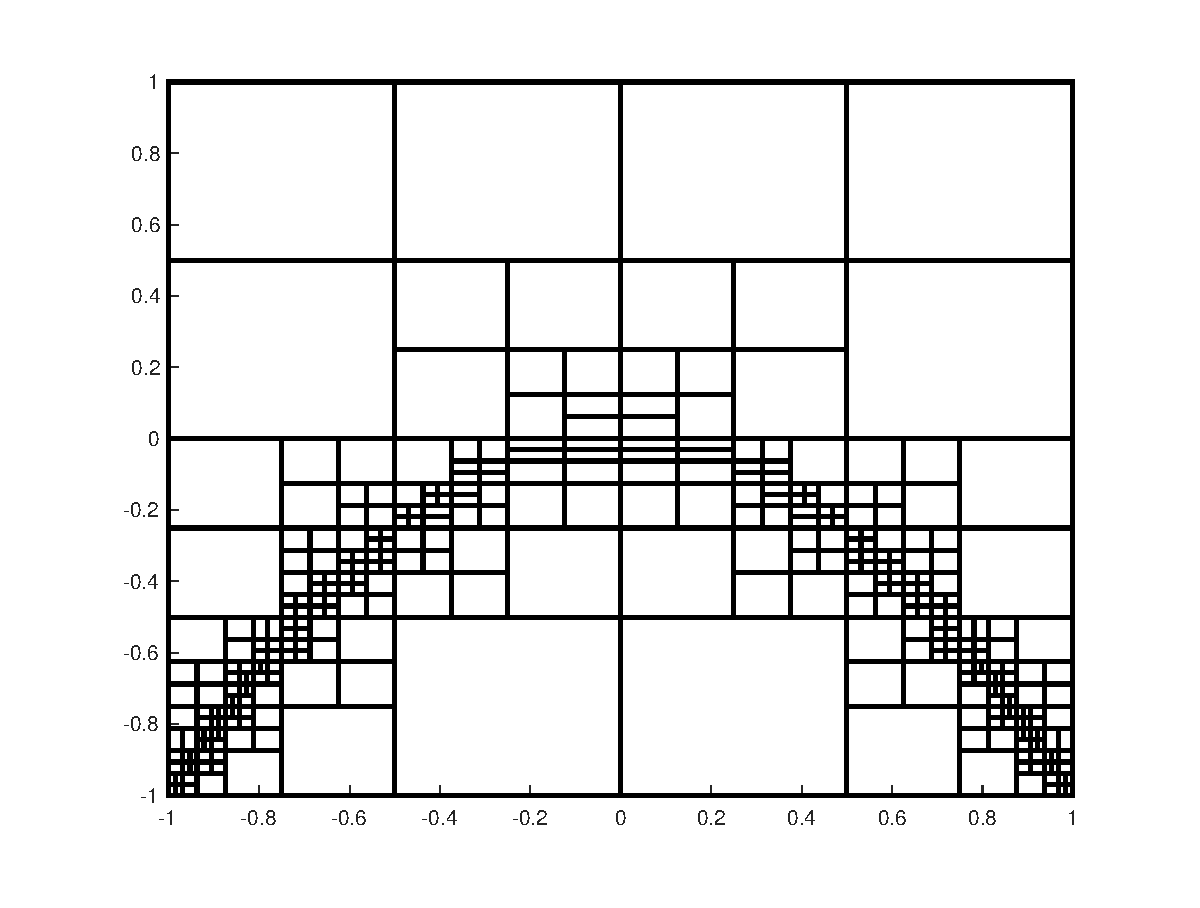
\includegraphics[scale = 0.3]{tan_100_1.eps}
   \label{zone_tan_a}
 }
\subfloat[Zone plot of $f_2(x,y)$]{
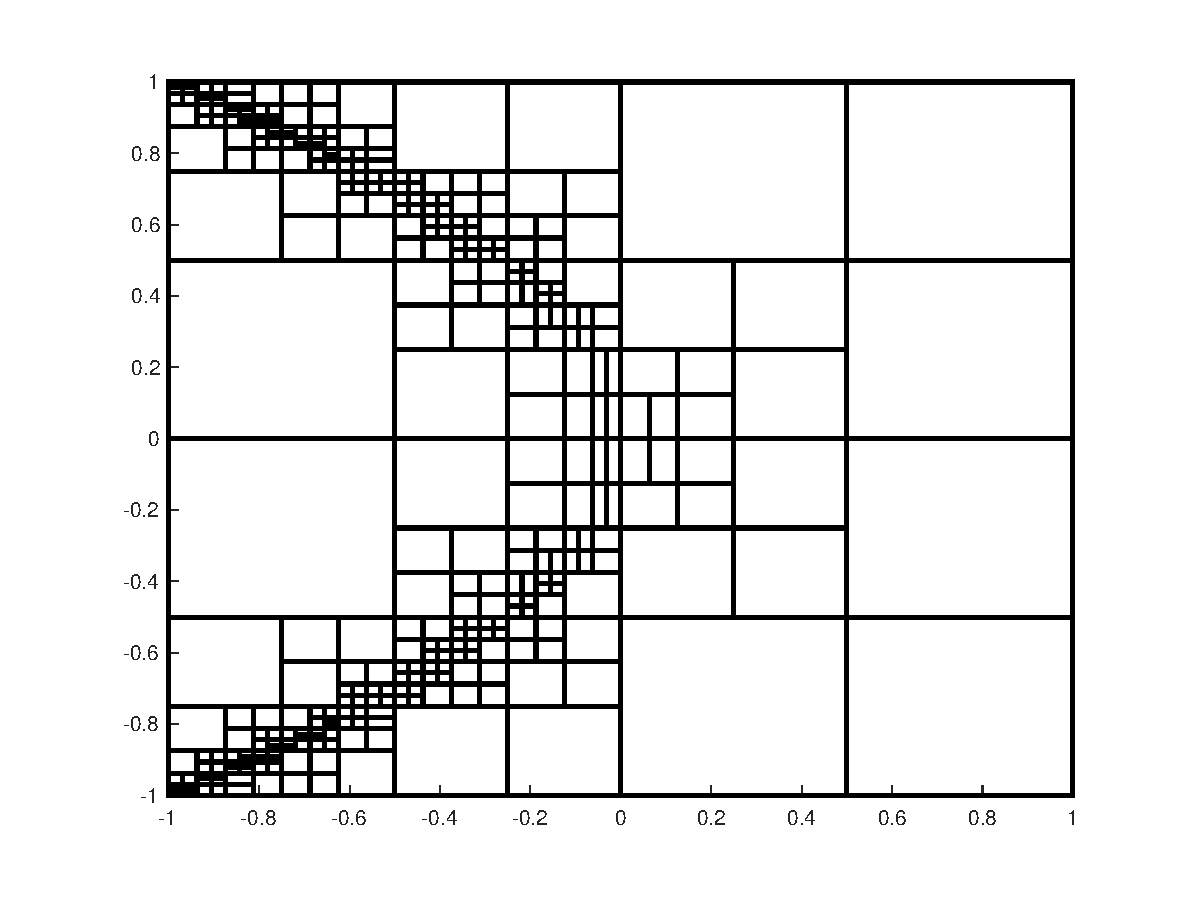
\includegraphics[scale = 0.3]{tan_100_2.eps}
   \label{zone_tan_b}
 }
 
 \subfloat[Zone plot of $f_1(x,y)+f_2(x,y)$]{
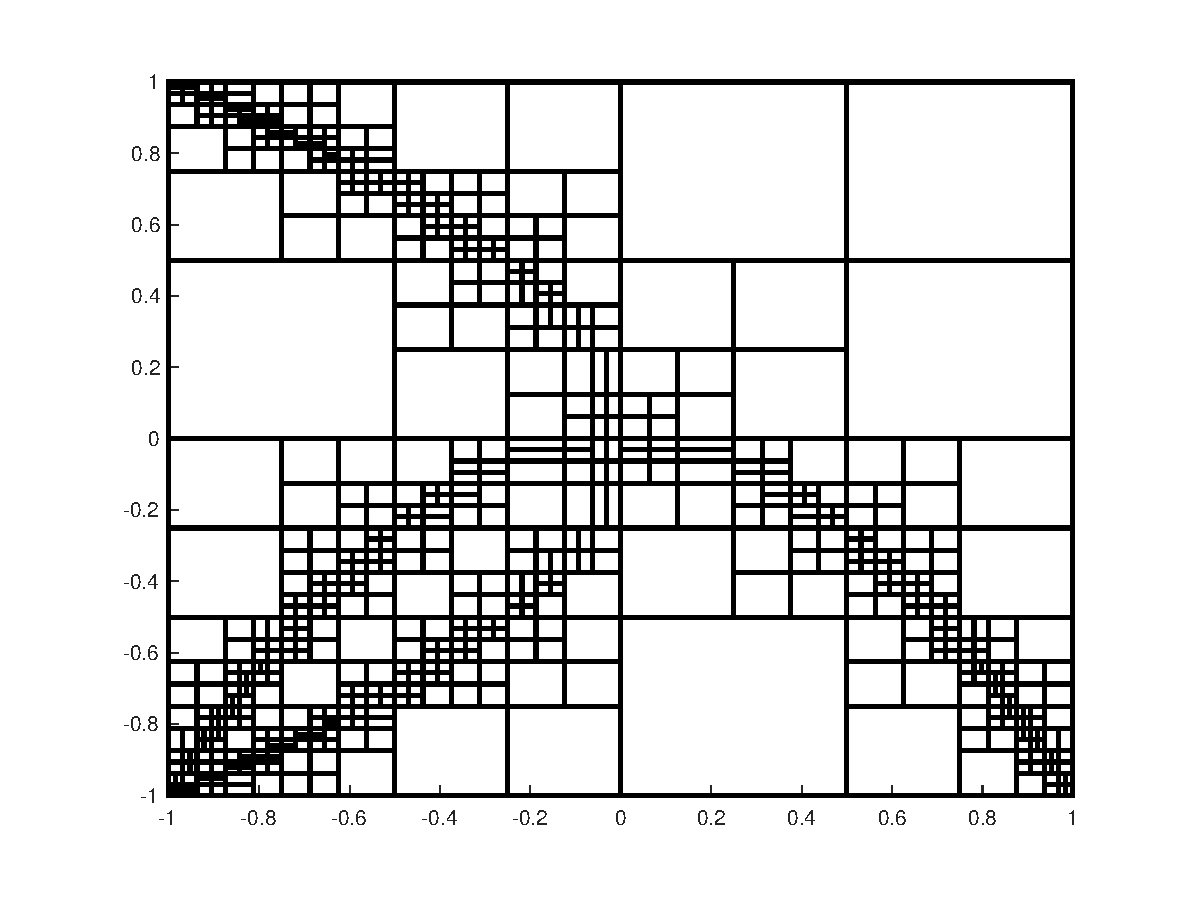
\includegraphics[scale = 0.3]{tan_100_3.eps}
   \label{zone_tan_c}
 }
 

\caption{Zone plots for $f_1(x,y)$,$f_2(x,y)$ and $f_1(x,y)+f_2(x,y)$.}
\label{zone_tan}
\end{figure}

\begin{figure}[!htb]
\centering
\subfloat[]{
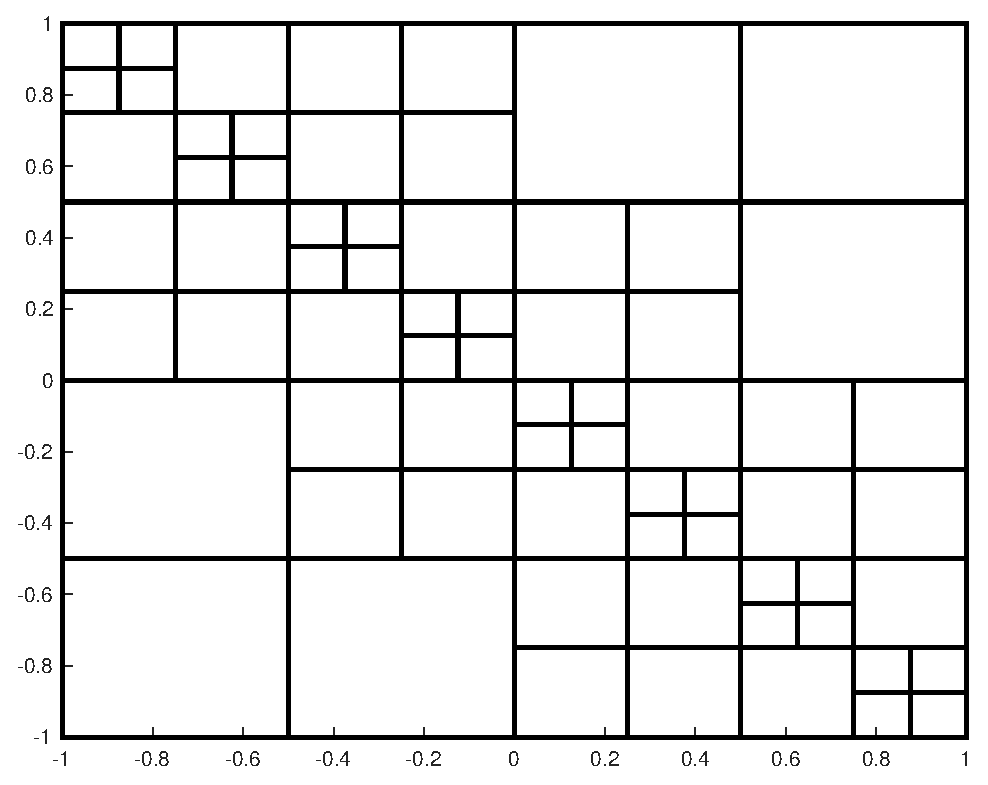
\includegraphics[scale = 0.3]{split_x.eps}
   \label{zone_tan_x}
 }
\subfloat[]{
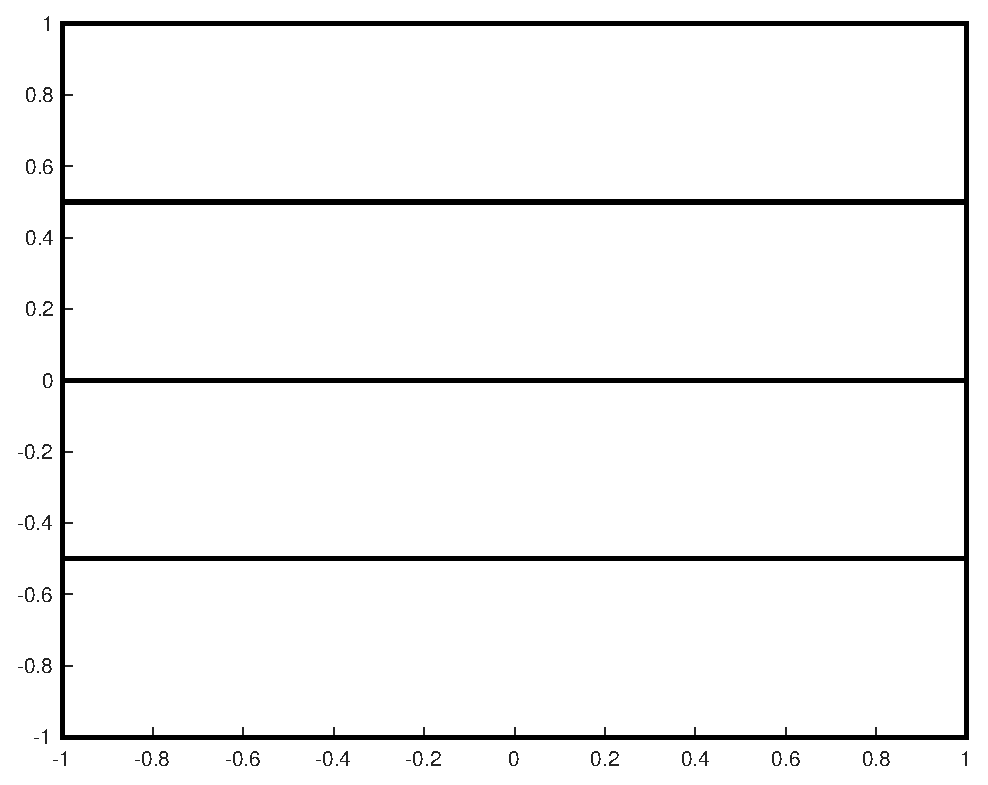
\includegraphics[scale = 0.3]{split_y.eps}
   \label{zone_tan_y}
 }


\caption{Example of two trees where recursion can not be used.}
\label{bad_split}
\end{figure}

\begin{algorithm}[!h]
\caption{$T$ = add($T_1$,$T_2$)}
\label{addition}
\begin{algorithmic}
\IF{$T_1$ is a leaf}
\STATE $T:=T_2$
\STATE for each leaf $\nu$ of $T$, add interpolant($T_1$) to interpolant($\nu$)
\ELSIF{$T_2$ is a leaf}
\STATE $T:=T_1$
\STATE for each leaf $\nu$ of $T$, add interpolant($T_2$) to interpolant($\nu$)
\ELSIF{splittingDim($T_1$)=splittingDim($T_2$)}
\STATE \child{0}($T$) = add(\child{0}($T_1$),\child{0}($T_2$))
\STATE \child{1}($T$) = add(\child{1}($T_1$),\child{1}($T_2$))
\ELSE
\STATE $T$=refine(max($T_1.\nmax,T_2.\nmax$),$T_1.t$,$T_1.\text{root.evalute}(x)+T_2.\text{root.evalute}(x)$)
\ENDIF
\end{algorithmic}
\end{algorithm}

\begin{algorithm}[!h]
\caption{$T$ = multiply($T_1$,$T_2$)}
\label{multiply}
\begin{algorithmic}
\IF{$T_1$ is a leaf}
\STATE $T:=T_2$
\STATE for each leaf $\nu$ of $T$, refine $\nu$ with $f(x)=\text{interpolant}(\nu)(x)\text{interpolant}(T_1)(x)$
\ELSIF{$T_2$ is a leaf}
\STATE $T:=T_1$
\STATE $T:=T_2$
\STATE for each leaf $\nu$ of $T$, refine $\nu$ with $f(x)=\text{interpolant}(\nu)(x)\text{interpolant}(T_2)(x)$
\ELSIF{splittingDim($T_1$)=splittingDim($T_2$)}
\STATE \child{0}($T$) = multiply(\child{0}($T_1$),\child{0}($T_2$))
\STATE \child{1}($T$) = multiply(\child{1}($T_1$),\child{1}($T_2$))
\ELSE
\STATE $T$=refine(max($T_1.\nmax,T_2.\nmax$),$T_1.t$,$T_1.\text{root.evalute}(x)T_2.\text{root.evalute}(x)$)
\ENDIF
\end{algorithmic}
\end{algorithm}

\section{Faster methods for adding and multiplying PU approximations}

Here we attempt to increase the speed of the addition and multiplication methods from before. There are two key differences here:
\begin{enumerate}
\item Here the new tree is created with recursive splits rather than by copying the subtrees,
\item and we add a case for dealing with trees where the splitting dimension does not match.	
\end{enumerate}
If we have a tree with uniform splitting (such as a 1D tree, or a 2D tree where leaves are always split in quarters), then the first four cases of Algorithm~\ref{addition2} will suffice. Suppose that we have trees $T_1$, $T_2$ that are first split in $x$ and $y$ respectively, and none of the children of $T_2$ are split in $x$. A simple example can be seen in Figure~\ref{bad_split_2}. In this case we would split $T_{\mbox{add}}$ along the $x$ dimension, as seen in the fifth case of Algorithm~\ref{addition2}. We then add \child{0}($T_1$) with $T_2$ and \child{1}($T_1$) with $T_2$. Since $T_2$ has no splits in $x$, we can assume that any subsequent splits of $T_{\mbox{add}}$ in Algorithm~\ref{addition2} will match that of $T_1$ and $T_2$ (i.e., the dividing hyperplanes will be the same). 

For our trees,
\begin{enumerate}
\item we always split in order ($x$-$y$ in 2D, $x$-$y$-$z$ in 3D),
\item and if a tree stops splitting in a dimension at any node, then no child of the node will split in that dimension.
\end{enumerate}
In 2D we can then see that the first 5 cases in Algorithm~\ref{addition2} will suffice. Suppose that we have two trees $T_1$, $T_2$ where the splitting dimensions don't match, and in the previous step in the recursion the trees split in $y$. In this case $nextSplit$ in Algorithm~\ref{addition2} will be in the $x$ direction. If $T_1$, $T_2$ split in $x,y$ respectively, then we know that $T_2$ does not split in $x$ direction anymore since the $x$ split was skipped (there were two splits in $y$ in a row). Since $T_2$ only splits in $y$, at any other point of the recursion where $nextSplit$ is in the $x$ direction we know the fifth case of Algorithm~\ref{addition2} will hold true. We have found this to work well in 3D, and have not found a case where the first 5 cases do not suffice. For example, adding the numerically approximations for
\begin{equation}
f_1(x,y,z) = \arctan(10(x+y)+z), \quad f_2(x,y,z) = \arctan(10(x+z)+y)
\end{equation}
only took 3 seconds; it takes 15 seconds to build an approximation for $f_1+f_2$ from scratch. We've included a failsafe step to ensure the algorithm does not fail for good measure.



\begin{figure}[!htb]
\centering
\subfloat[]{
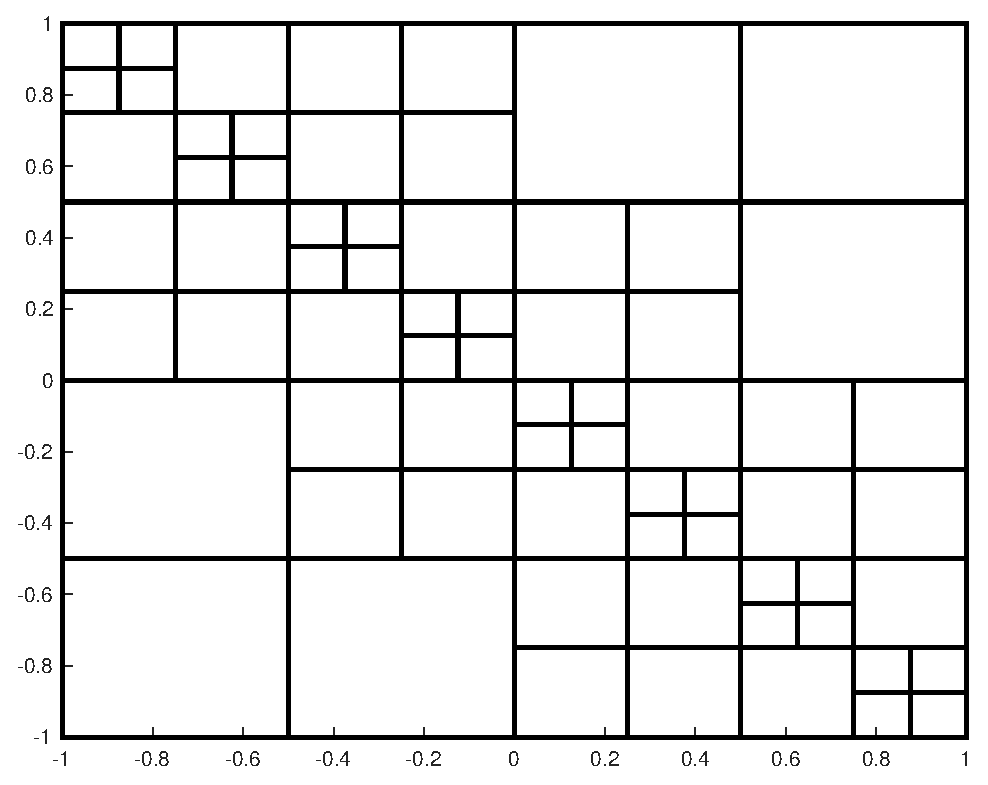
\includegraphics[scale = 0.3]{split_x.eps}
   \label{zone_tan_x}
 }
\subfloat[]{
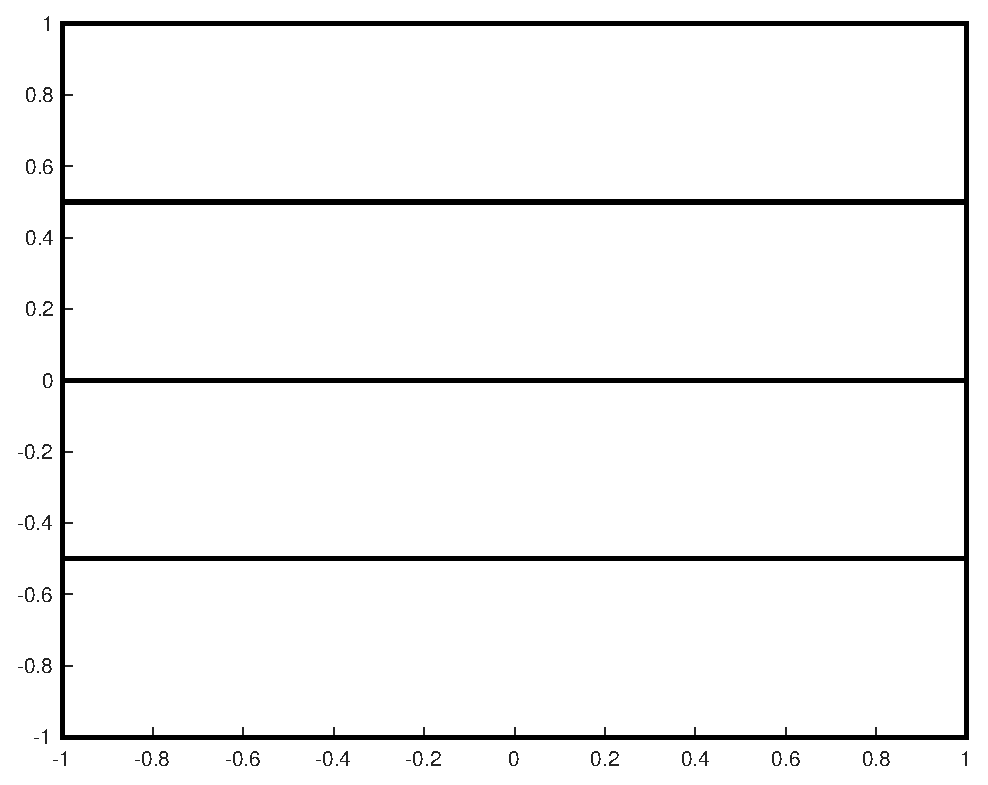
\includegraphics[scale = 0.3]{split_y.eps}
   \label{zone_tan_y}
 }

\caption{Example of two trees with different splittings.}
\label{bad_split_2}
\end{figure}

\begin{algorithm}[!h]
\caption{$T_{\mbox{add}}$ = add($T_1$,$T_2$,$T_{\mbox{add}}$,$split$)}
\label{addition2}
\begin{algorithmic}
\IF{$T_1$ and $T_2$ are leaves}
\STATE interpolant($T_{\mbox{add}}$)=interpolant($T_1$)+interpolant($T_2$) on domain($T_{\mbox{add}}$).
\ELSIF{$T_1$ is a leaf while $T_2$ is not}
\STATE split($T_{\mbox{add}}$,$T_1$.splitDim,$T_2$.overlap)
\STATE \child{0}($T_{\mbox{add}}$)=add($T_1$,\child{0}($T_2$),\child{0}($T_{\mbox{add}}$),$T_2$.splitDim)
\STATE \child{1}($T_{\mbox{add}}$)=add($T_1$,\child{1}($T_2$),\child{1}($T_{\mbox{add}}$),$T_2$.splitDim)
\ELSIF{$T_1$ is not a leaf while $T_2$ is}
\STATE split($T_{\mbox{add}}$,$T_1$.splitDim,$T_1$.overlap)
\STATE \child{0}($T_{\mbox{add}}$)=add(\child{0}($T_1$),$T_2$,\child{0}($T_{\mbox{add}}$),$T_1$.splitDim)
\STATE \child{1}($T_{\mbox{add}}$)=add(\child{1}($T_1$),$T_2$,\child{1}($T_{\mbox{add}}$),$T_1$.splitDim)
\ELSIF{$T_1$.splitDim=$T_2$.splitDim}
\STATE split($T_{\mbox{add}}$,$T_1$.splitDim,$T_1$.overlap)
\STATE \child{0}($T_{\mbox{add}}$)=add(\child{0}($T_1$),\child{0}($T_2$),\child{0}($T_{\mbox{add}}$),$T_1$.splitDim)
\STATE \child{1}($T_{\mbox{add}}$)=add(\child{1}($T_1$),\child{1}($T_2$),\child{1}($T_{\mbox{add}}$),$T_1$.splitDim)
\ELSE
\STATE Let $nextSplit$ be the next ordered split after $split$ from $T_1$.splitDim, $T_2$.splitDim
\IF{$nextSplit$=$T_1$.splitDim and $T_2$ does not split in $T_1$.splitDim anymore}
\STATE split($T_{\mbox{add}}$,$T_1$.splitDim,$T_1$.overlap)
\STATE \child{0}($T_{\mbox{add}}$)=add(\child{0}($T_1$),$T_2$,\child{0}($T_{\mbox{add}}$),$T_1$.splitDim)
\STATE \child{1}($T_{\mbox{add}}$)=add(\child{1}($T_1$),$T_2$,\child{1}($T_{\mbox{add}}$),$T_1$.splitDim)
\ELSIF{$nextSplit$=$T_2$.splitDim and $T_1$ does not split in $T_2$.splitDim anymore}
\STATE split($T_{\mbox{add}}$,$T_1$.splitDim,$T_1$.overlap)
\STATE \child{0}($T_{\mbox{add}}$)=add($T_1$,\child{0}($T_2$),\child{0}($T_{\mbox{add}}$),$T_1$.splitDim)
\STATE \child{1}($T_{\mbox{add}}$)=add($T_1$,\child{1}($T_2$),\child{1}($T_{\mbox{add}}$),$T_1$.splitDim)
\ELSE
\STATE $T_{\mbox{add}}$=refine(max($T_1.\nmax,T_2.\nmax$),$T_1$.overlap,$T_1(x)+T_2(x)$)
\ENDIF
\ENDIF
\end{algorithmic}
\end{algorithm}

\begin{algorithm}[!h]
\caption{$T_{\mbox{add}}$ = multiply($T_1$,$T_2$,$T_{\mbox{add}}$,$split$)}
\label{addition2}
\begin{algorithmic}
\IF{$T_1$ and $T_2$ are leaves}
\STATE $T_{\mbox{add}}$=refine(max($T_1.\nmax,T_2.\nmax$),$T_1$.overlap,$T_1(x)T_2(x)$) on domain($T_{\mbox{add}}$).
\ELSIF{$T_1$ is a leaf while $T_2$ is not}
\STATE split($T_{\mbox{add}}$,$T_1$.splitDim,$T_2$.overlap)
\STATE \child{0}($T_{\mbox{add}}$)=multiply($T_1$,\child{0}($T_2$),\child{0}($T_{\mbox{add}}$),$T_2$.splitDim)
\STATE \child{1}($T_{\mbox{add}}$)=multiply($T_1$,\child{1}($T_2$),\child{1}($T_{\mbox{add}}$),$T_2$.splitDim)
\ELSIF{$T_1$ is not a leaf while $T_2$ is}
\STATE split($T_{\mbox{add}}$,$T_1$.splitDim,$T_1$.overlap)
\STATE \child{0}($T_{\mbox{add}}$)=multiply(\child{0}($T_1$),$T_2$,\child{0}($T_{\mbox{add}}$),$T_1$.splitDim)
\STATE \child{1}($T_{\mbox{add}}$)=multiply(\child{1}($T_1$),$T_2$,\child{1}($T_{\mbox{add}}$),$T_1$.splitDim)
\ELSIF{$T_1$.splitDim=$T_2$.splitDim}
\STATE split($T_{\mbox{add}}$,$T_1$.splitDim,$T_1$.overlap)
\STATE \child{0}($T_{\mbox{add}}$)=multiply(\child{0}($T_1$),\child{0}($T_2$),\child{0}($T_{\mbox{add}}$),$T_1$.splitDim)
\STATE \child{1}($T_{\mbox{add}}$)=multiply(\child{1}($T_1$),\child{1}($T_2$),\child{1}($T_{\mbox{add}}$),$T_1$.splitDim)
\ELSE
\STATE Let $nextSplit$ be the next ordered split after $split$ from $T_1$.splitDim, $T_2$.splitDim
\IF{$nextSplit$=$T_1$.splitDim and $T_2$ does not split in $T_1$.splitDim anymore}
\STATE split($T_{\mbox{add}}$,$T_1$.splitDim,$T_1$.overlap)
\STATE \child{0}($T_{\mbox{add}}$)=multiply(\child{0}($T_1$),$T_2$,\child{0}($T_{\mbox{add}}$),$T_1$.splitDim)
\STATE \child{1}($T_{\mbox{add}}$)=multiply(\child{1}($T_1$),$T_2$,\child{1}($T_{\mbox{add}}$),$T_1$.splitDim)
\ELSIF{$nextSplit$=$T_2$.splitDim and $T_1$ does not split in $T_2$.splitDim anymore}
\STATE split($T_{\mbox{add}}$,$T_1$.splitDim,$T_1$.overlap)
\STATE \child{0}($T_{\mbox{add}}$)=multiply($T_1$,\child{0}($T_2$),\child{0}($T_{\mbox{add}}$),$T_1$.splitDim)
\STATE \child{1}($T_{\mbox{add}}$)=multiply($T_1$,\child{1}($T_2$),\child{1}($T_{\mbox{add}}$),$T_1$.splitDim)
\ELSE
\STATE $T_{\mbox{add}}$=refine(max($T_1.\nmax,T_2.\nmax$),$T_1$.overlap,$T_1(x)T_2(x)$)
\ENDIF
\ENDIF
\end{algorithmic}
\end{algorithm}

\section{Addition take 3}


From Algorithm~\ref{addition3}, we see that there are 5 cases to check for:
\begin{enumerate}
\item Both $T_1$ and $T_2$ are leaves,
\item $T_1$ is a leaf but $T_2$ is not,
\item $T_1$ is not a leaf but $T_2$ is,
\item $T_1$ and $T_2$ are both not leaves and immediately split in the same dimension,
\item $T_1$ and $T_2$ are both not leaves, and if $T_k$ immediately splits in dim $split$, then the other tree does not for any of its children.
\end{enumerate}
This list is not logically exhaustive, so we must prove inductively that these five cases hold. If we have two leaves, there is nothing to prove. If $T_1$ is a leaf and $T_2$ is not, then only cases 1-2 can hold for $T_1$ and \child{k}($T_2$); this is similarly true if $T_2$ is a leaf and $T_1$ is not. Suppose we have case 4 with $T_1$ and $T_2$ for $split$, and for \child{k}($T_1$), \child{k}($T_2$) cases 1-4 are false. If $\text{\child{k}}(T_1).\text{splitDim}=nextsplit$ in Algorithm~\ref{addition3}, then it must be the case that $\text{\child{k}}(T_2)$ stops splitting entirely for dimensions $T_2.\text{splitDim}+1,\dots,\text{\child{k}}(T_1).\text{splitDim},\dots,\text{\child{k}}(T_2).\text{splitDim}-1$. Thus the fifth case holds for \child{k}($T_1$) and \child{k}($T_2$).

Suppose now we have reached the fifth case of Algorithm~\ref{addition3}, where $T_1.\text{splitDim}=nextsplit$, and for \child{k}($T_1$), $T_2$ cases 1-4 fail. We first reach this case either from the first call, or from a recursive call from case 4. In any case, we can assume that $T_2$ stops splitting entirely for dimensions $T_1.\text{splitDim},\dots,T_2.\text{splitDim}-1$; this is the induction hypothesis we will use to argue that with subsequent calls of Algorithm~\ref{addition3} from case 5 that $T_1$, $T_2$ must satisfy one of the cases. If we have $\text{\child{k}}(T_1).\text{splitDim}<T_2.\text{splitDim}$, we know that then that $nextsplit$=\child{k}($T_1$).splitDim and by assumption that $T_2$ does not split in $\text{\child{k}}(T_1).\text{splitDim},\dots,T_2.\text{splitDim}-1$, hence case 5 is true and the induction hypothesis is satisfied. Next suppose that $\text{\child{k}}(T_1)>T_2.\text{splitDim}$. We can know that $\text{\child{k}}(T_1)$ stops splitting entirely for dimensions $T_1.\text{splitDim}+1,\dots,T_2.\text{splitDim},\dots,\text{\child{k}}(T_1).\text{splitDim}-1$. In this case we see that $nextsplit=T_2.\text{splitDim}$, so case 5 and the induction hypothesis hold. We thus have by induction that in any point in the recursion, only cases 1-5 can hold.

\section{Addition take 4: putting it all together}

Suppose we have two PU approximations $\hat{s}_1(\vect{x})$, $\hat{s}_2(\vect{x})$, represented by trees $T_1$ and $T_2$ respectively. The simplest approach to building a PU approximation of $sum(\vect{x})=\hat{s}_1(\vect{x})+\hat{s}_2(\vect{x})$ is to add patch by patch if $T_1$ and $T_2$ share the same leaves, or use Algorithm~\ref{alg3} with $sum(\vect{x})$ otherwise. The cost of sampling $sum(\vect{x})$ can be expensive though; to evaluate an $n^{d}$ grid with a $d$-dimensional Chebyshev interpolant of max degree $n$ requires $O(n^{d+1})$ computations (while taking advantage of the grid structure). Thus by predetermining the needed splitting to approximate $sum(\vect{x})$, we can greatly reduce the cost of the numerical addition. As an example we build approximations for
\begin{equation}
f_1(x,y) = \arctan(100(x^2+y)), \quad f_2(x,y) = \arctan(100(x+y^2)),
\end{equation}
as well as $f_1(x,y)+f_2(x,y)$. It can readily be observed that the splitting of $f_1(x,y)+f_2(x,y)$ is a merging of that of $f_1(x,y)$ and $f_2(x,y)$. Algorithm~\ref{addition3} adds the approximations by first producing a tree $T_{\text{add}}$ with a merged splitting of the different approximations; at the initial call of Algorithm~\ref{addition3}, $T_{\text{add}}$ is a single leaf.


\begin{figure}[!htb]
\centering
\subfloat[Zone plot of $f_1(x,y)$]{
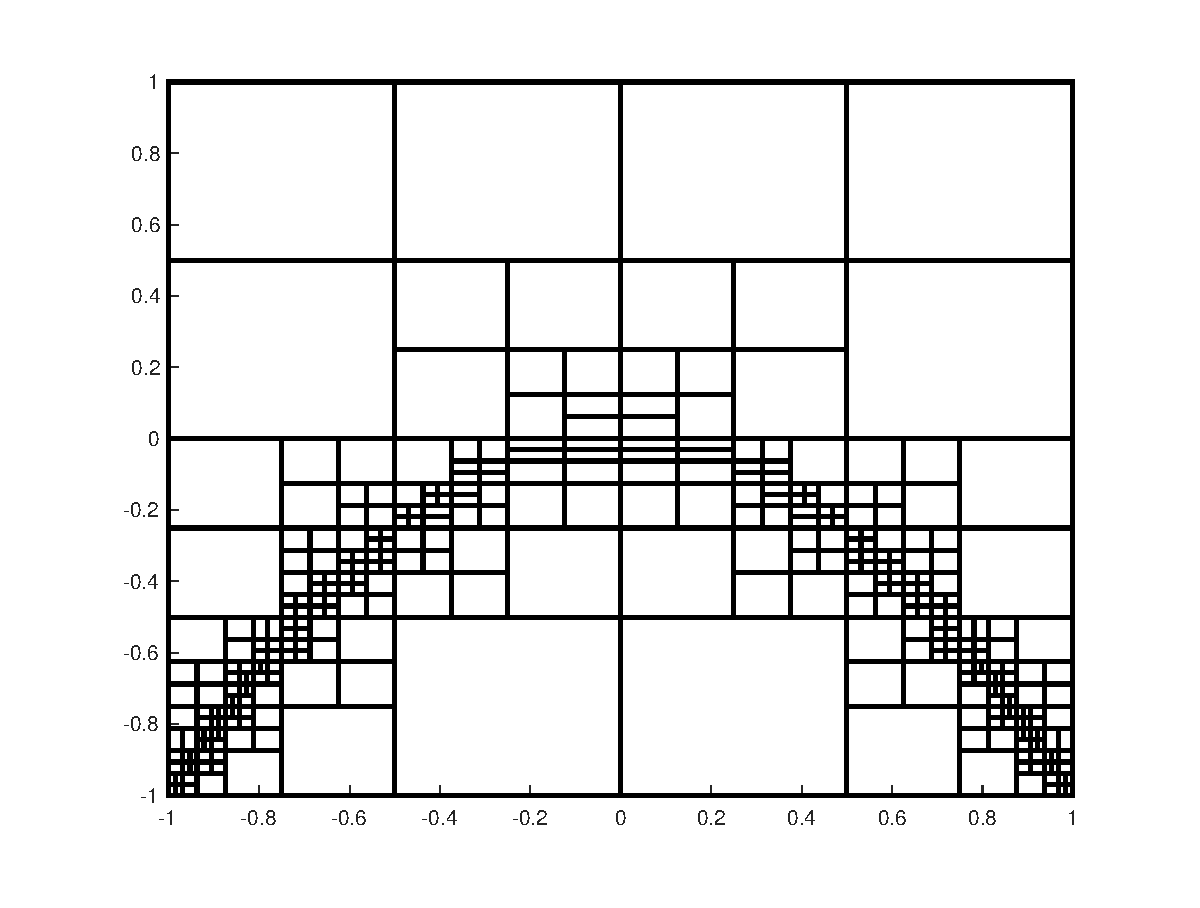
\includegraphics[scale = 0.3]{tan_100_1.eps}
   \label{zone_tan_a}
 }
\subfloat[Zone plot of $f_2(x,y)$]{
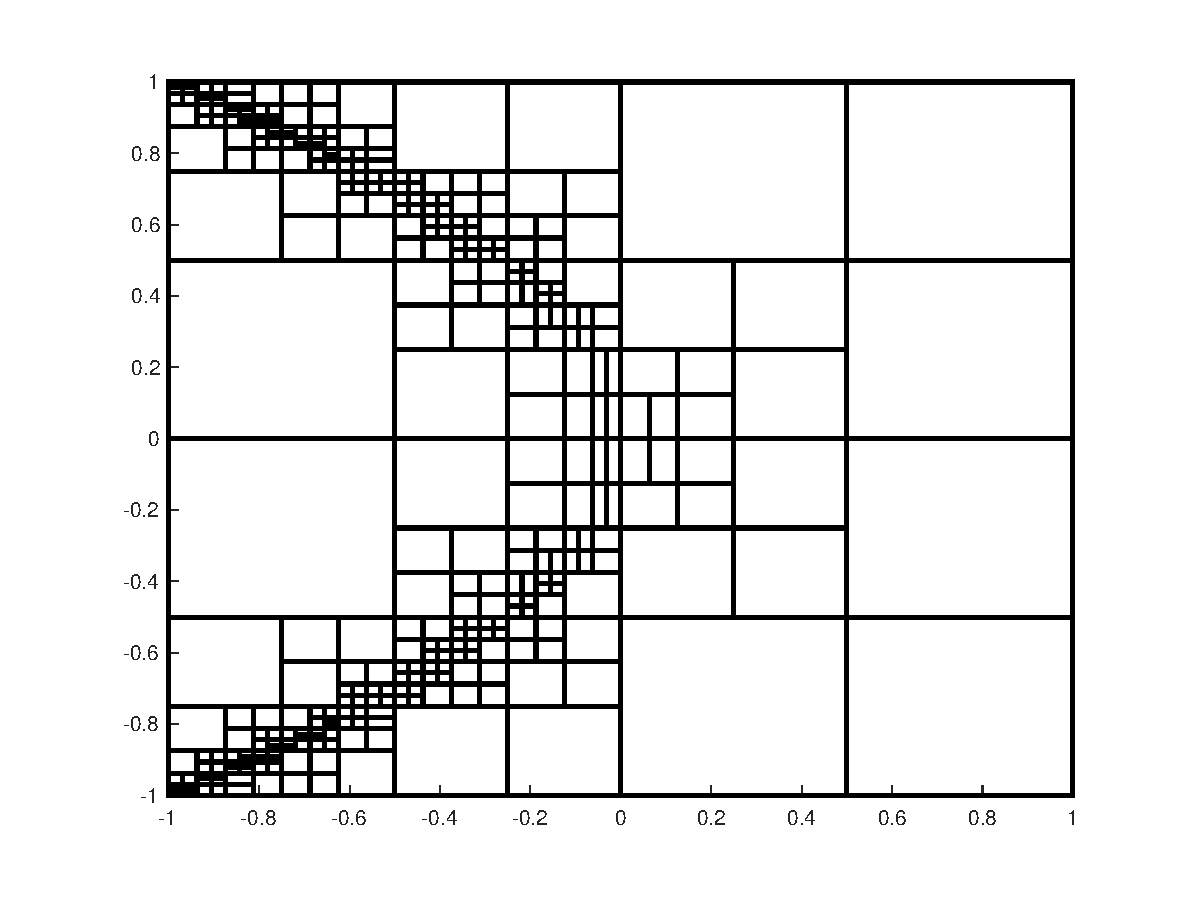
\includegraphics[scale = 0.3]{tan_100_2.eps}
   \label{zone_tan_b}
 }
 
 \subfloat[Zone plot of $f_1(x,y)+f_2(x,y)$]{
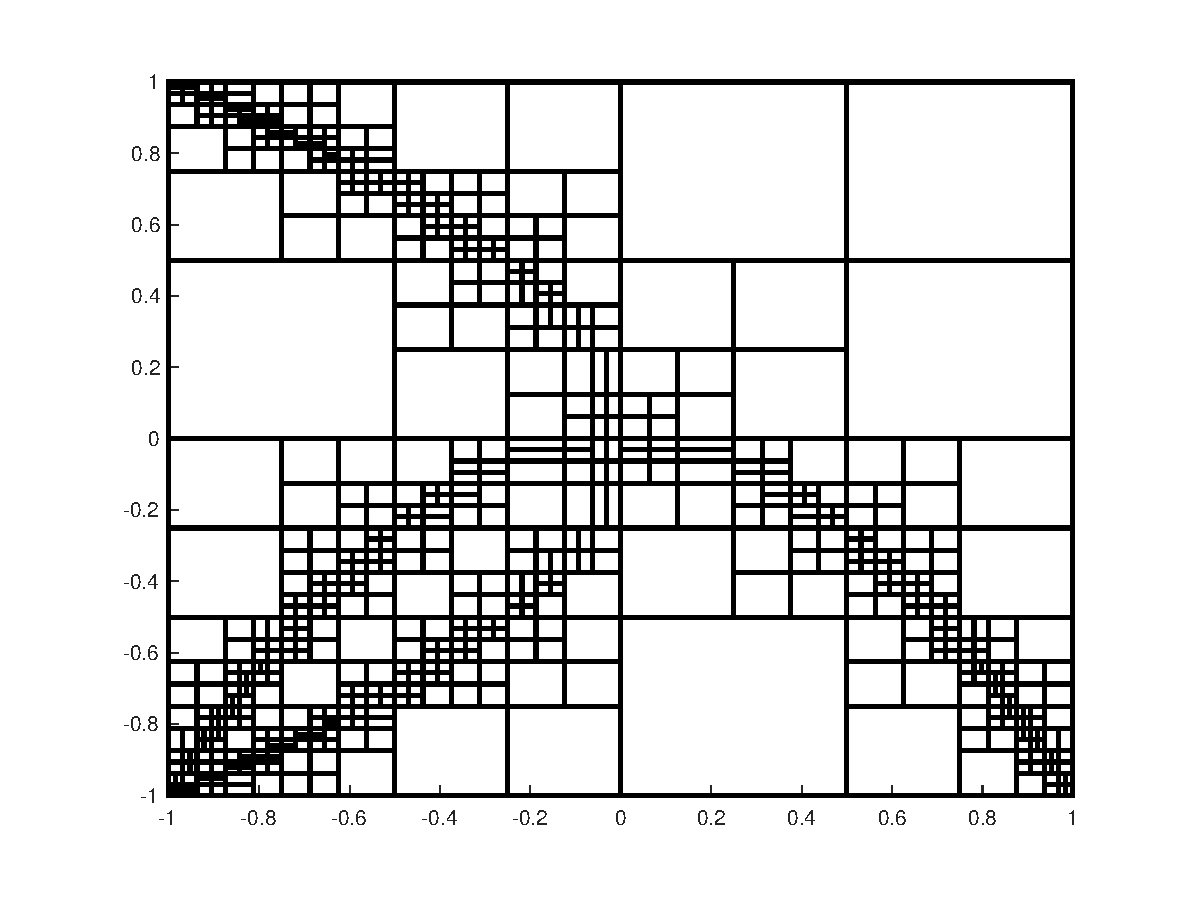
\includegraphics[scale = 0.3]{tan_100_3.eps}
   \label{zone_tan_c}
 }
 \caption{Zone plots for $f_1(x,y)$,$f_2(x,y)$ and $f_1(x,y)+f_2(x,y)$.}
\label{zone_tan}
\end{figure}
 
 \begin{figure}[!htb]
\centering
\subfloat[]{
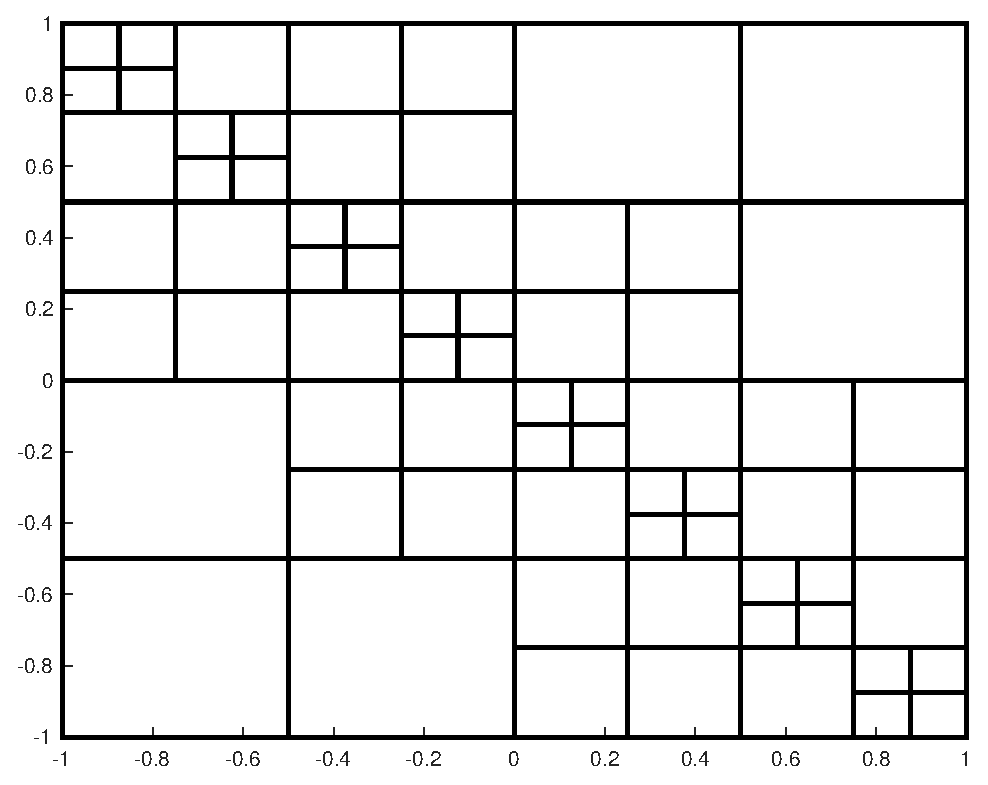
\includegraphics[scale = 0.3]{split_x.eps}
   \label{zone_tan_1}
 }
\subfloat[]{
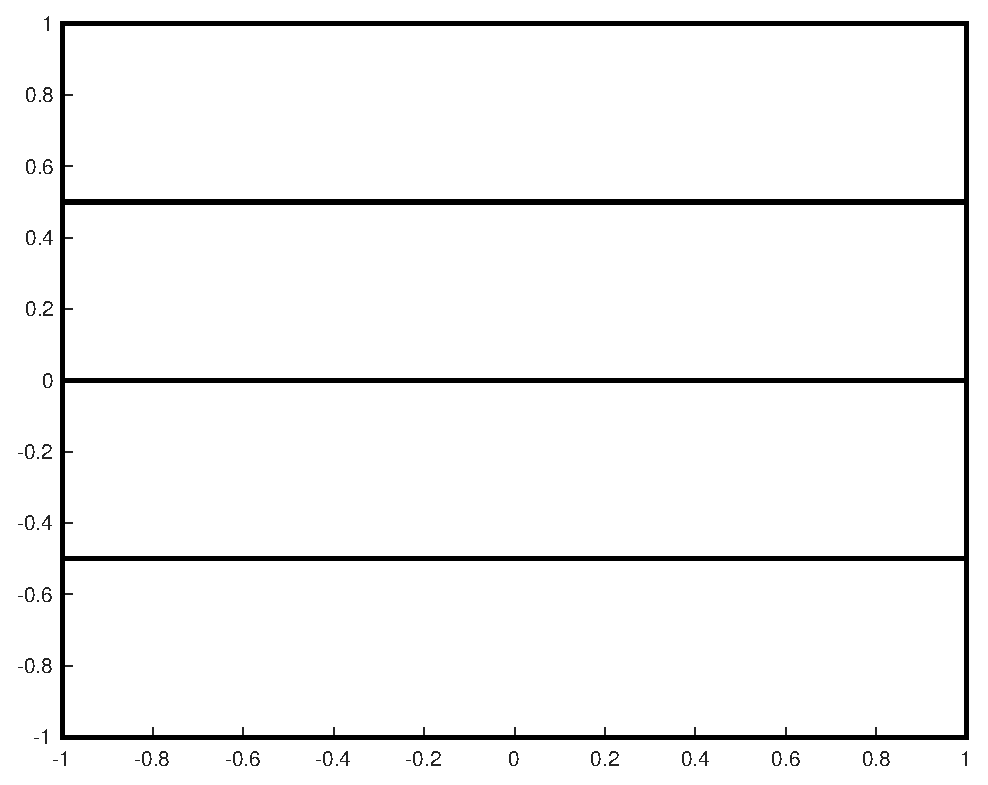
\includegraphics[scale = 0.3]{split_y.eps}
   \label{zone_tan_2}
 }
\caption{Example of two trees where the initial split does not match}
\label{bad_split}
\end{figure}

If $\hat{s}_1(\vect{x})$, $\hat{s}_2(\vect{x})$ are 1D approximations, only the first four cases of Algorithm~\ref{addition3} are needed, and it is clear that $T_{\text{add}}$ is a tree with a merged splitting of $T_1$ and $T_2$. Suppose $T_1$ and $T_2$ produce zones as seen in Figures~\ref{zone_tan_1}-\ref{zone_tan_2}. Here we have that splitDim($T_1$)=x, splitDim($T_2$)=y, and $T_2$ only splits in $y$. Since this is first call $nextSplit=x$. This means in Algorithm~\ref{addition3} we would split $T_{\mbox{add}}$ in the $x$ direction, and call add(\child{k}($T_1$),$T_2$,\child{k}($T_{\mbox{add}}$)) for $k=1,2$.  We see that $T_2$ is fully needed to cover the zones of both \child{1}($T_1$),\child{2}($T_1$) since $T_2$ does not split in $x$. Furthermore, even though the domains of \child{k}($T_{\mbox{add}}$) and $T_2$ don't match, the length in the $y$-dimension is the same; this is enough to ensure that further splittings of $T_{\mbox{add}}$ in the $y$ direction will match that of $T_2$. In this case, Algorithm~\ref{addition3} would produce a merged splitting of the two trees. It is the case that this holds when the splitting dimensions don't match, as seen in Theorem~\ref{split_theorem}.  A key fact of this proof is that for our trees
\begin{enumerate}
\item we always split in order ($x$-$y$ in 2D, $x$-$y$-$z$ in 3D),
\item and if a tree stops splitting in a dimension at any node, then no child of the node will split in that dimension.
\end{enumerate} 
Thus if we have a tree $T$ where splitDim($T$)=$d_1$ and splitDim(\child{0}($T$))=$d_k$, we then know that $T$ skipped dimensions $d_2,\dots,d_{k-1}$; this means that \child{0}($T$) can not split in these dimensions at all. We use this fact to prove Theorem~\ref{split_theorem} inductively.


\begin{theorem}
Suppose in Algorithm~\ref{addition3} that 
\begin{equation}
\text{splitDim($T_1$)} \neq \text{splitDim($T_2$)}, \quad nextsplit=\text{splitDim($T_1$)}.
\label{split_assump}
\end{equation}
Then $T_2$ stops splitting in dimension splitDim($T_1$). 
\label{split_theorem}
\end{theorem}

\begin{proof}
For the different cases where (\ref{split_assump}) occurs we argue with specific dimensions; the proofs can be easily generalized. Suppose that we are at the fist call where
\begin{equation}
 \text{splitDim($T_1$)}=d_1 , \quad \text{splitDim($T_2$)}=d_k
\end{equation}
with $k>1$. In Algorithm~\ref{addition3} $nextsplit=d_1$ because we are at the first call. Since $T_2$ starts splitting in $d_k$, it does not split in $d_1,\dots,d_{k-1}$. The next case to consider is when 
\begin{equation}
\text{splitDim($T_1$)}=\text{splitDim($T_2$)}, \quad \text{splitDim(\child{k}($T_1$))} \neq \text{splitDim(\child{k}($T_2$))}.
\end{equation}
Suppose here that
\begin{equation}
\text{splitDim($T_1$)}=d_n, \quad \text{splitDim(\child{k}($T_1$))}=d_1, \quad \text{splitDim(\child{k}($T_2$))}=d_k.
\end{equation}
such that $k>1$. Again $nextsplit=d_1$, and we see that $T_2$ has skipped past dimensions $d_1,d_2,\dots,d_{k-1}$. This implies that splitDim(\child{k}($T_2$)) stops splitting in these dimensions as well.

Finally suppose that 
\begin{equation}
\text{splitDim($T_1$)} \neq \text{splitDim($T_2$)}, \quad  \text{splitDim(\child{k}($T_1$))} \neq \text{splitDim($T_2$)},
\end{equation}
where with $T_1$ and $T_2$ we have $nextsplit=\text{splitDim($T_1$)}$. The first time that the fifth case of Algorithm~\ref{addition3} can occur is if we are at the first call, or if in the previous call the splitting dimension matched between the trees. In either case, we would have $T_2$ does not split in dimensions $\text{splitDim($T_1$)}+1,\dots,\text{splitDim($T_2$)}-1$. We claim this remains true with successive calls of the fifth case, and will prove so inductively. Suppose that with splitDim(\child{k}($T_1$)) and splitDim($T_2$) that $nextsplit=\text{splitDim(\child{k}($T_1$))}$. This implies splitDim(\child{k}($T_1$)) lies between splitDim($T_1$) and splitDim($T_2$); by assumption we have $T_2$ does not split in $\text{splitDim(\child{k}($T_1$))}+1,\dots,\text{splitDim($T_2$)}-1$ so the induction hypothesis holds. If $nextsplit=\text{splitDim($T_2$)}$, then we know that $T_1$ skipped dimensions $\text{splitDim($T_1$)},\dots,\text{splitDim($T_2$)},\dots,\text{splitDim(\child{k}($T_1$))}-1$ implying the induction hypothesis holds in this case as well for \child{k}($T_1$). This shows that with successive calls of the fifth case of Algorithm~\ref{addition3} starting from the first call or the fourth case that if splitDim($T_1$)$\neq$splitDim($T_2$) and $nextsplit$=splitDim($T_1$), then $T_2$ stops splitting in splitDim($T_1$).

\end{proof}

\begin{algorithm}[!h]
\caption{add($T_1$,$T_2$,$T_{\mbox{add}}$,$LastSplit$)}
\label{addition3}
\begin{algorithmic}
\IF{$T_1$ and $T_2$ are leaves}
\STATE interpolant($T_{\mbox{add}}$)=interpolant($T_1$)+interpolant($T_2$) on domain($T_{\mbox{add}}$).
\ELSIF{$T_1$ is a leaf while $T_2$ is not}
\STATE split($T_{\mbox{add}}$,$T_1$.splitDim,$T_2$.overlap)
\STATE add($T_1$,\child{0}($T_2$),\child{0}($T_{\mbox{add}}$),$T_2$.splitDim)
\STATE add($T_1$,\child{1}($T_2$),\child{1}($T_{\mbox{add}}$),$T_2$.splitDim)
\ELSIF{$T_1$ is not a leaf while $T_2$ is}
\STATE split($T_{\mbox{add}}$,$T_1$.splitDim,$T_1$.overlap)
\STATE add(\child{0}($T_1$),$T_2$,\child{0}($T_{\mbox{add}}$),$T_1$.splitDim)
\STATE add(\child{1}($T_1$),$T_2$,\child{1}($T_{\mbox{add}}$),$T_1$.splitDim)
\ELSIF{$T_1$.splitDim=$T_2$.splitDim}
\STATE split($T_{\mbox{add}}$,$T_1$.splitDim,$T_1$.overlap)
\STATE add(\child{0}($T_1$),\child{0}($T_2$),\child{0}($T_{\mbox{add}}$),$T_1$.splitDim)
\STATE add(\child{1}($T_1$),\child{1}($T_2$),\child{1}($T_{\mbox{add}}$),$T_1$.splitDim)
\ELSE
\STATE $nextsplit=(LastSplit \mod \text{dim($T_1$)}) +1$
\WHILE{$T_1$.splitDim $\neq nextsplit$ and $T_2$.splitDim $\neq nextsplit$}
\STATE $nextsplit=(nextsplit \mod \text{dim($T_1$)}) +1$
\ENDWHILE
\STATE split($T_{\mbox{add}}$,$nextsplit$,$T_2$.overlap)
\IF{$T_1$.splitDim=$nextsplit$}
\STATE add(\child{0}($T_1$),$T_2$,\child{0}($T_{\mbox{add}}$),$nextsplit$)
\STATE add(\child{1}($T_1$),$T_2$,\child{1}($T_{\mbox{add}}$),$nextsplit$)
\ELSE
\STATE add($T_1$,\child{0}($T_2$),\child{0}($T_{\mbox{add}}$),$nextsplit$)
\STATE add($T_1$,\child{1}($T_2$),\child{1}($T_{\mbox{add}}$),$nextsplit$)
\ENDIF
\ENDIF
\end{algorithmic}
\end{algorithm}

\bibliographystyle{plain}
\bibliography{PU_BIB}

\end{document}